\documentclass[aspectratio=169]{beamer}
\mode<presentation>{
  \usetheme{default}
  \usecolortheme{dove}
}
\defbeamertemplate*{footline}{my footline}
{
	\ifnum \insertpagenumber=1
		\leavevmode%
		
\includegraphics[width=\paperwidth]{MPIM_Titelseite_unten.pdf}%NEW
		\vskip-10pt%NEW
		\hbox{%
			\pgfsetfillopacity{0}\begin{beamercolorbox}[wd=1\paperwidth,ht=2.25ex,dp=1ex,center]{title in head/foot}%
				\usebeamerfont{title in head/foot}\pgfsetfillopacity{1}%\insertframenumber{} / \inserttotalframenumber\hspace*{2ex}
			\end{beamercolorbox}%
		}%
		\vskip0pt%
	\else
		\leavevmode%
		%
\includegraphics[width=\paperwidth]{MPIM_IMPRS_Folgeseite_unten.pdf}
		
\includegraphics[width=\paperwidth]{MPIM_Titelseite_unten.pdf}		
		\vskip-10pt
		\hbox{%
			\pgfsetfillopacity{0}\begin{beamercolorbox}[wd=1\paperwidth,ht=2.25ex,dp=1ex,center]{title in head/foot}%
				\usebeamerfont{title in head/foot}\pgfsetfillopacity{1}\insertframenumber{} / \inserttotalframenumber\hspace*{2ex}
			\end{beamercolorbox}%
		}%
		\vskip0pt%
	\fi
}
%\usepackage{pgfpages}
%\setbeameroption{show notes on second screen=right}
\setbeamertemplate{navigation symbols}{}%remove navigation symbols

%\usepackage[colorlinks=true, urlcolor=blue, linkcolor=blue,citecolor=blue]{hyperref}
%\usepackage[german]{babel}
\usepackage{tikz}
\usepackage{float}
%\usepackage[numbers]{natbib}
\usepackage[authoryear]{natbib}
\definecolor{links}{HTML}{2A1B81}
\hypersetup{colorlinks,linkcolor=links,urlcolor=links}
\usepackage{appendixnumberbeamer}
\usepackage[font=footnotesize,labelfont=bf]{caption}
%\let\oldcite=\cite                                                              
%\renewcommand{\cite}[1]{\textcolor[rgb]{.7,.7,.7}{\oldcite{#1}}}

\usepackage{graphicx}
\graphicspath{{/home/mpim/m300524/MSc_Thesis/gfx/}}

%\newcommand{\memberpositive}{m105_1994_2001}
\newcommand{\memberpositive}{m178_1985_1992} % zweitbesten
%\newcommand{\memberpositive}{m182_1988_1995} %funktioniert am besten

\renewcommand\refname{References and Notes}


\makeatletter
\setbeamertemplate{footline}[my footline]





%\title{\vspace{1cm} \\ Internal variability of the Southern Ocean carbon sink in MPI-ESM large ensemble simulations: perspective from responses of ocean biology and circulation to westerly wind changes}
\title{\vspace{5mm} \\ Decadal variations in the Southern Ocean carbon sink in MPI-ESM 100 ensemble simulations}%: \\ assessment of westerly wind changes}

\subtitle{ \vspace{1cm} Aaron Spring,$^{1}$ Hongmei Li,$^{1}$ Tatiana Ilyina$^{1}$
\\ \normalsize{$^{1}$Max Planck Institute for Meteorology, Bundesstra{\ss}e 53, 20146 Hamburg, Germany}
}



\begin{document}
\begin{frame}[noframenumbering]
	\titlepage
\end{frame}

\section{Introduction}

\begin{frame}{Southern Ocean carbon sink}% - Analysis of positive CO$_2$ flux trend}

\begin{figure}[h]
	\begin{minipage}{.5\textwidth}
		\centering
			%\vspace{-2mm}
			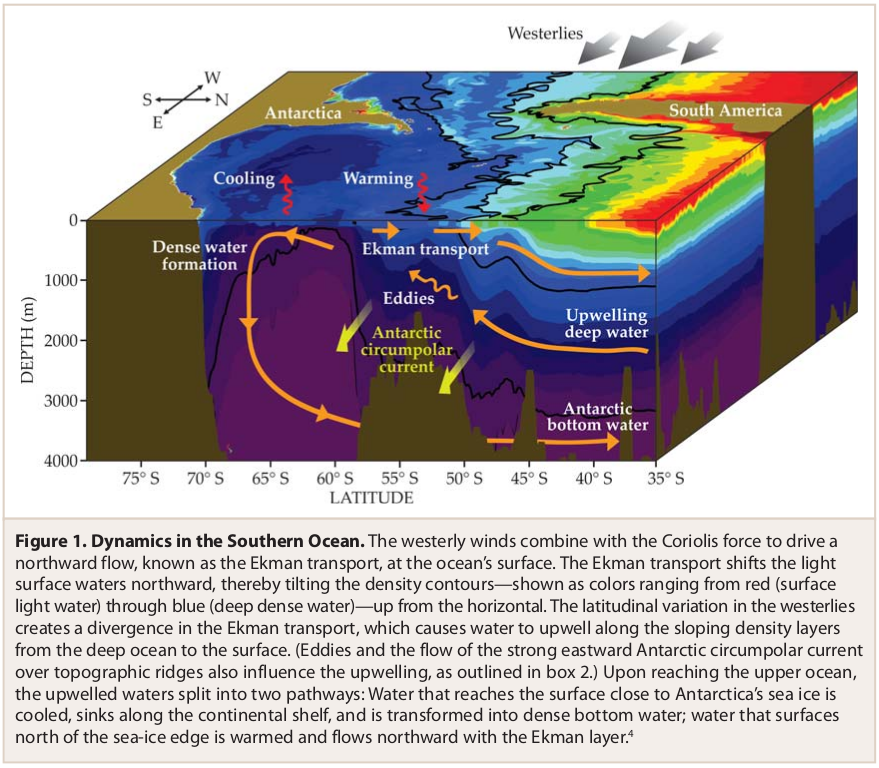
\includegraphics[scale=.45,trim=.3cm 6.8cm .5cm .5cm,clip]{Southern_Ocean_Circulation}
\vspace{-2mm}
	\caption{Dynamics of the Southern Ocean \citep{Morrison2015}}
		\label{fig:SO_review}
	\end{minipage} \hfill
	\begin{minipage}{.25\textwidth}

		Ocean-side changes in CO$_2$ flux:		
		\begin{itemize}
			\item thermal
			\item circulation
			\item biology
		\end{itemize}
		\hspace{-1cm}
	
		
	\end{minipage}
\end{figure}
\vspace{-12mm}

\begin{flushright}
$\text{CO}_2\text{flux}=k_w \cdot  \underbrace{\left( pCO_\text{2,ocean} - pCO_\text{2,atm}\right)}_{\Delta pCO_2}	$
\end{flushright}

\end{frame}



\begin{frame}{Recent observations suggest pronounced decadal variations in the Southern Ocean carbon sink.}
\begin{minipage}{.11\textwidth}
\small \vspace{-1.5cm} anomalous outgassing \\ \\ \\ \\{anomalous uptake}
\end{minipage} \hfill 
	\begin{minipage}{.88\textwidth}
\begin{figure}[h]
	\centering
	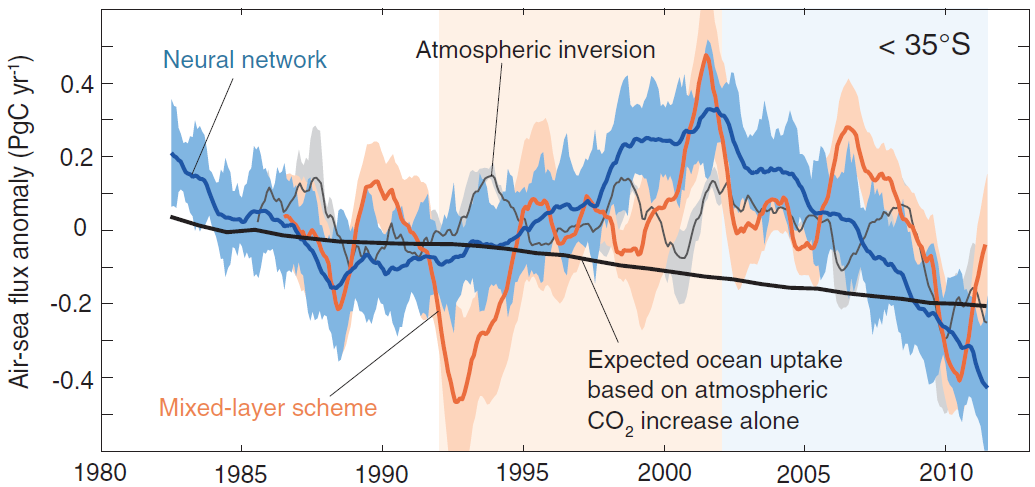
\includegraphics[scale=.315]{landschuetzer_fig1.png} % from gfx folder
\vspace{-1.5mm}	
	\caption{Evolution of the Southern Ocean carbon sink anomaly south of 35$^\circ$S. Negative CO$_2$flux values indicate anomalous ocean uptake with respect to the 1980s mean \citep{landschuetzer2015}.}
	\label{fig:landschuetzer_fig1}
\end{figure}
\end{minipage}
\end{frame}





\begin{frame}{However, due to the sparse spatial and temporal coverage, it is challenging to discern the dynamics of internally varying processes.}
\begin{figure}[h]
	\centering
	\begin{minipage}{.45\textwidth}
		\centering
		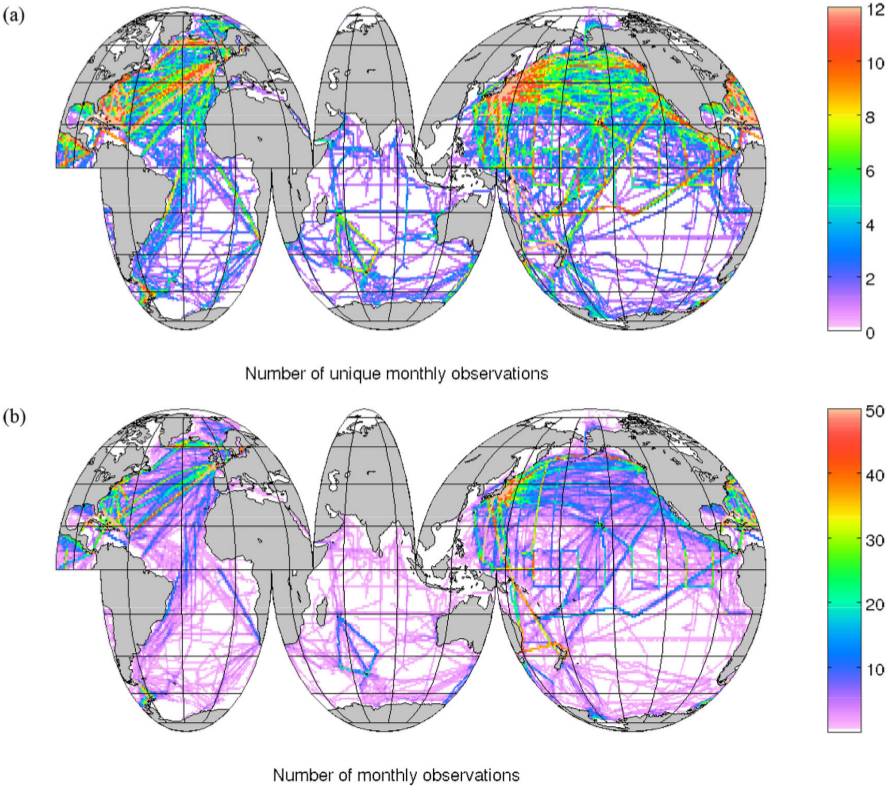
\includegraphics[scale=.225]{Bakker_fig8.png}
		\caption{The number of (a) months of the year and (b) total months with surface water pCO$_2$ from 1970 to 2011 in SOCATv2 \citep{Bakker2014}}
		\label{fig:Bakker_fig1}
	\end{minipage} \hfill \pause
	\begin{minipage}{.45\textwidth}
		\centering
		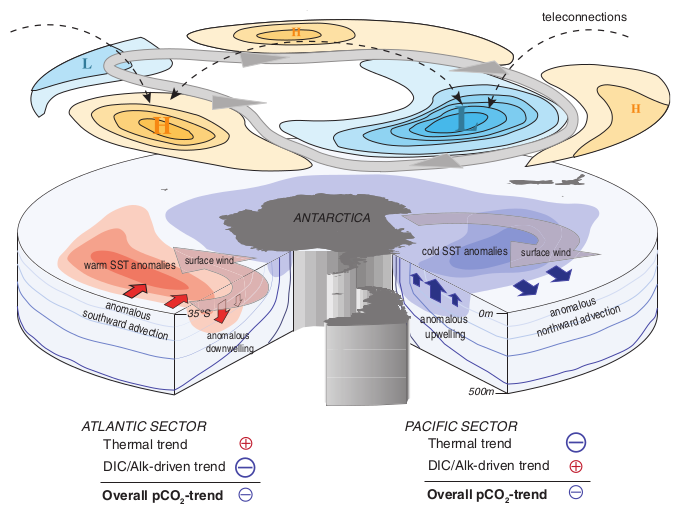
\includegraphics[scale=.3]{Landschuetzer2015_fig3.png} % from gfx folder
		\caption{Schematic of the processes governing the changes in $\Delta$pCO$_2$ trends in the Southern Ocean since 2001 \citep{landschuetzer2015}}
		\label{fig:landschuetzer_fig3}
	\end{minipage}
\end{figure}

\end{frame}


\begin{frame}{Earth system models, while being a useful tool to analyze processes that contribute to variability, do not always capture this variability.}

\begin{figure}[h]
	\centering
	\begin{minipage}{.45\textwidth}
		\centering
		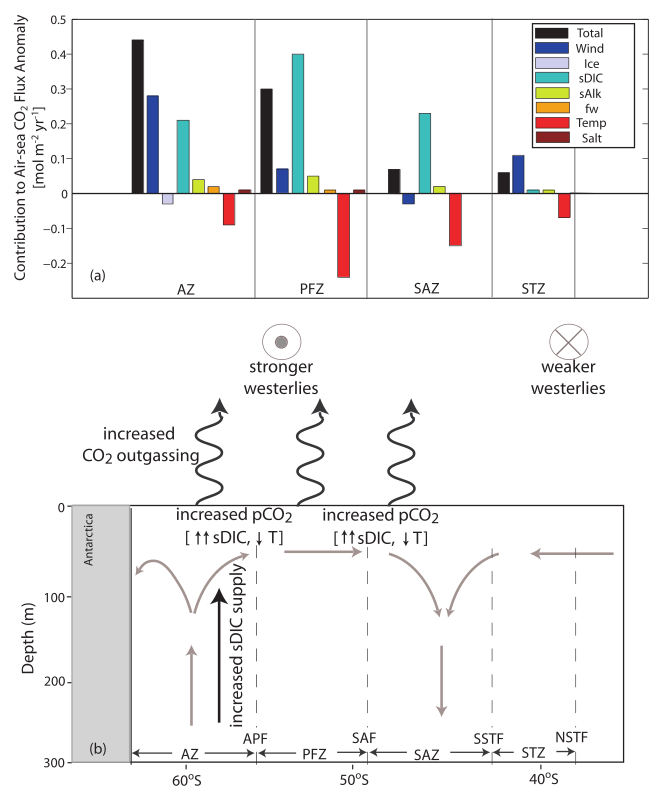
\includegraphics[scale=.225]{Lovenduski2007_fig9.png}
		\caption{Contribution to air-sea CO$_2$ flux anomaly and schematic illustration of the upper ocean response to a positive phase of the SAM \citep{Lovenduski2007}}
		\label{fig:Lovenduski_fig9}
	\end{minipage} \hfill \pause
	\begin{minipage}{.45\textwidth}
		\centering
		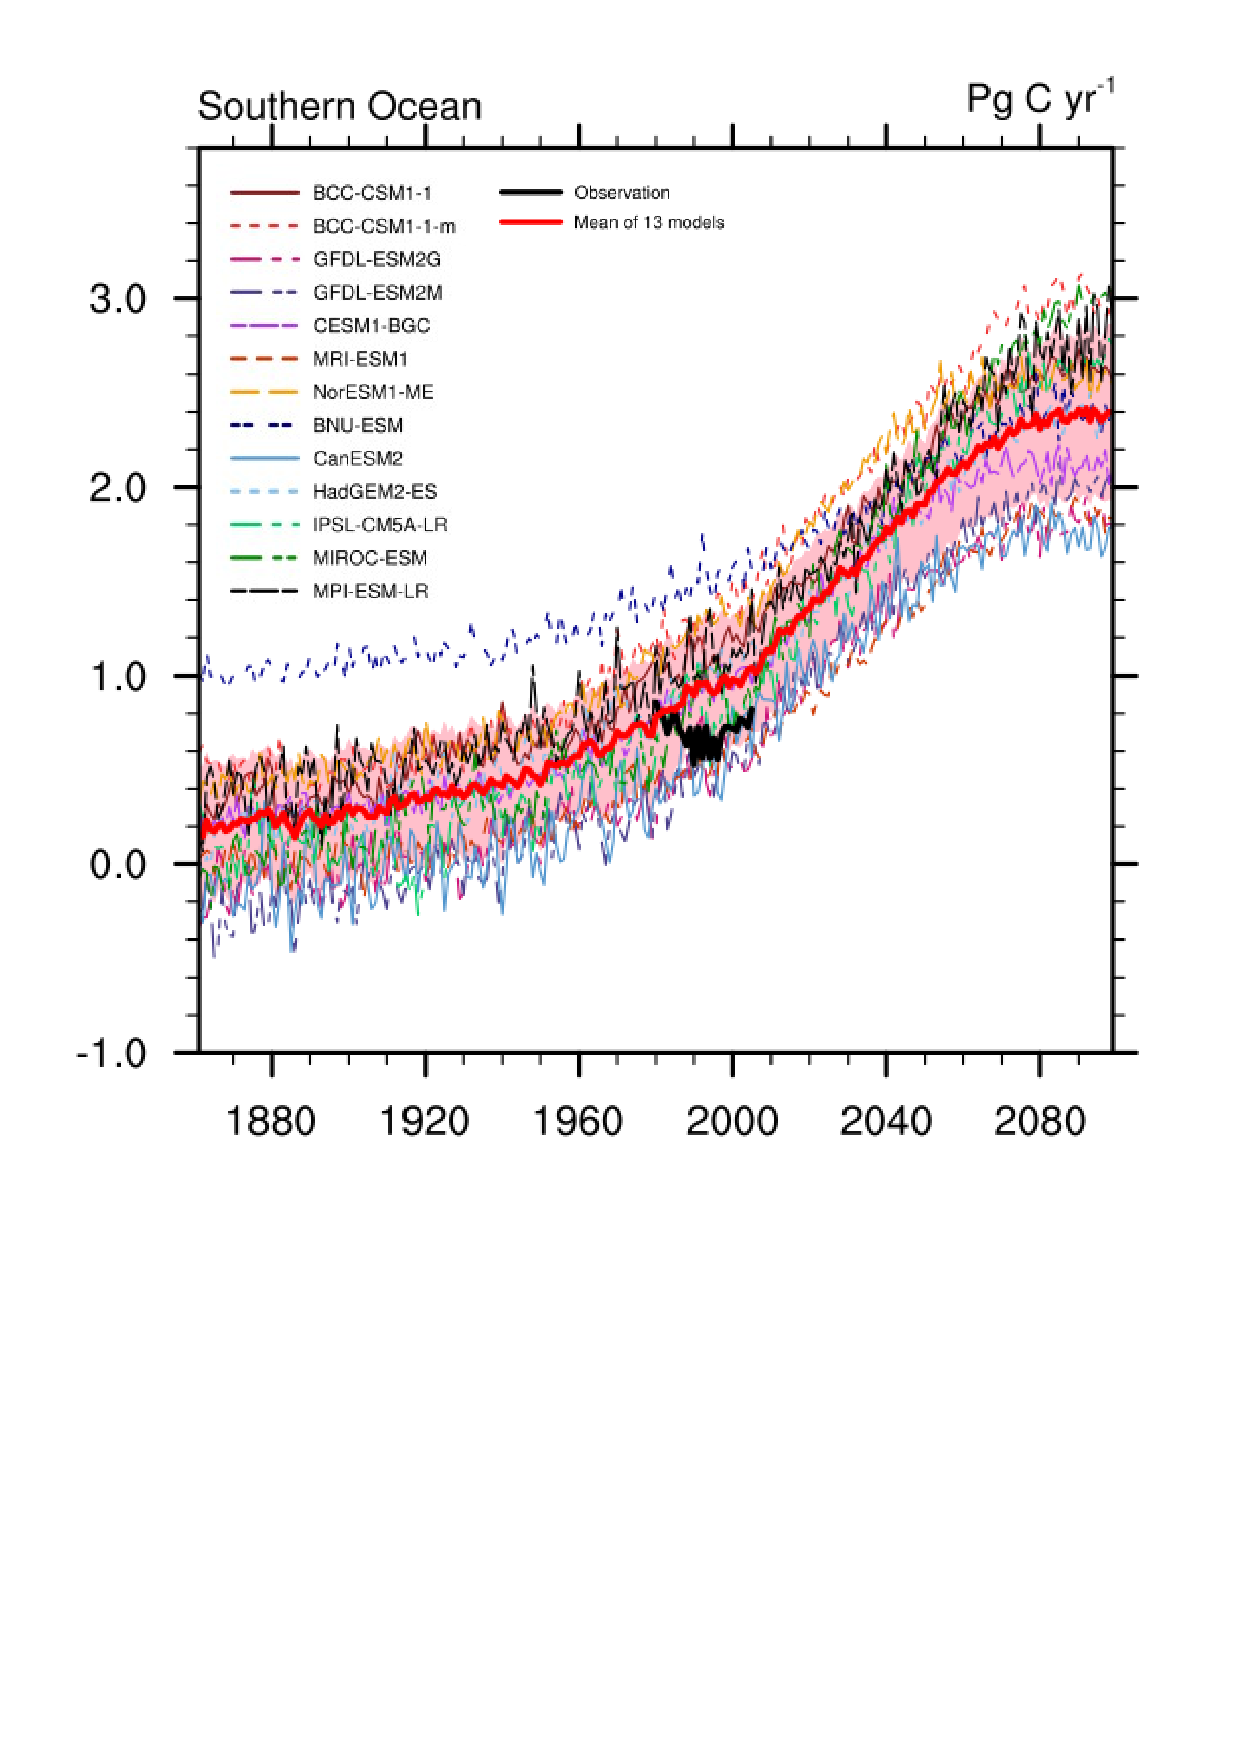
\includegraphics[scale=.27,trim=0cm 10.2cm 0cm 2.2cm,clip]{wang20161d.pdf} % from gfx folder
		\caption{Historical and projected total air-sea CO$_2$ fluxes in the Southern Ocean simulated by 13 CMIP5 models \citep{Wang2016}}
		\label{fig:Wang_fig1d}
	\end{minipage}
\end{figure}


\end{frame}

	
\section{Method}
\begin{frame}{By analyzing a large ensemble of 100 historical simulations based on Max Planck Institute Earth System Model (MPI-ESM) with slightly different initial conditions but identical forcing, we assess modeled internal variability of the Southern Ocean carbon sink.}
%I identify similar decadal trends in the MPI-ESM LE.	

	\begin{figure}
		\centering
		\begin{minipage}{.55\textwidth}
		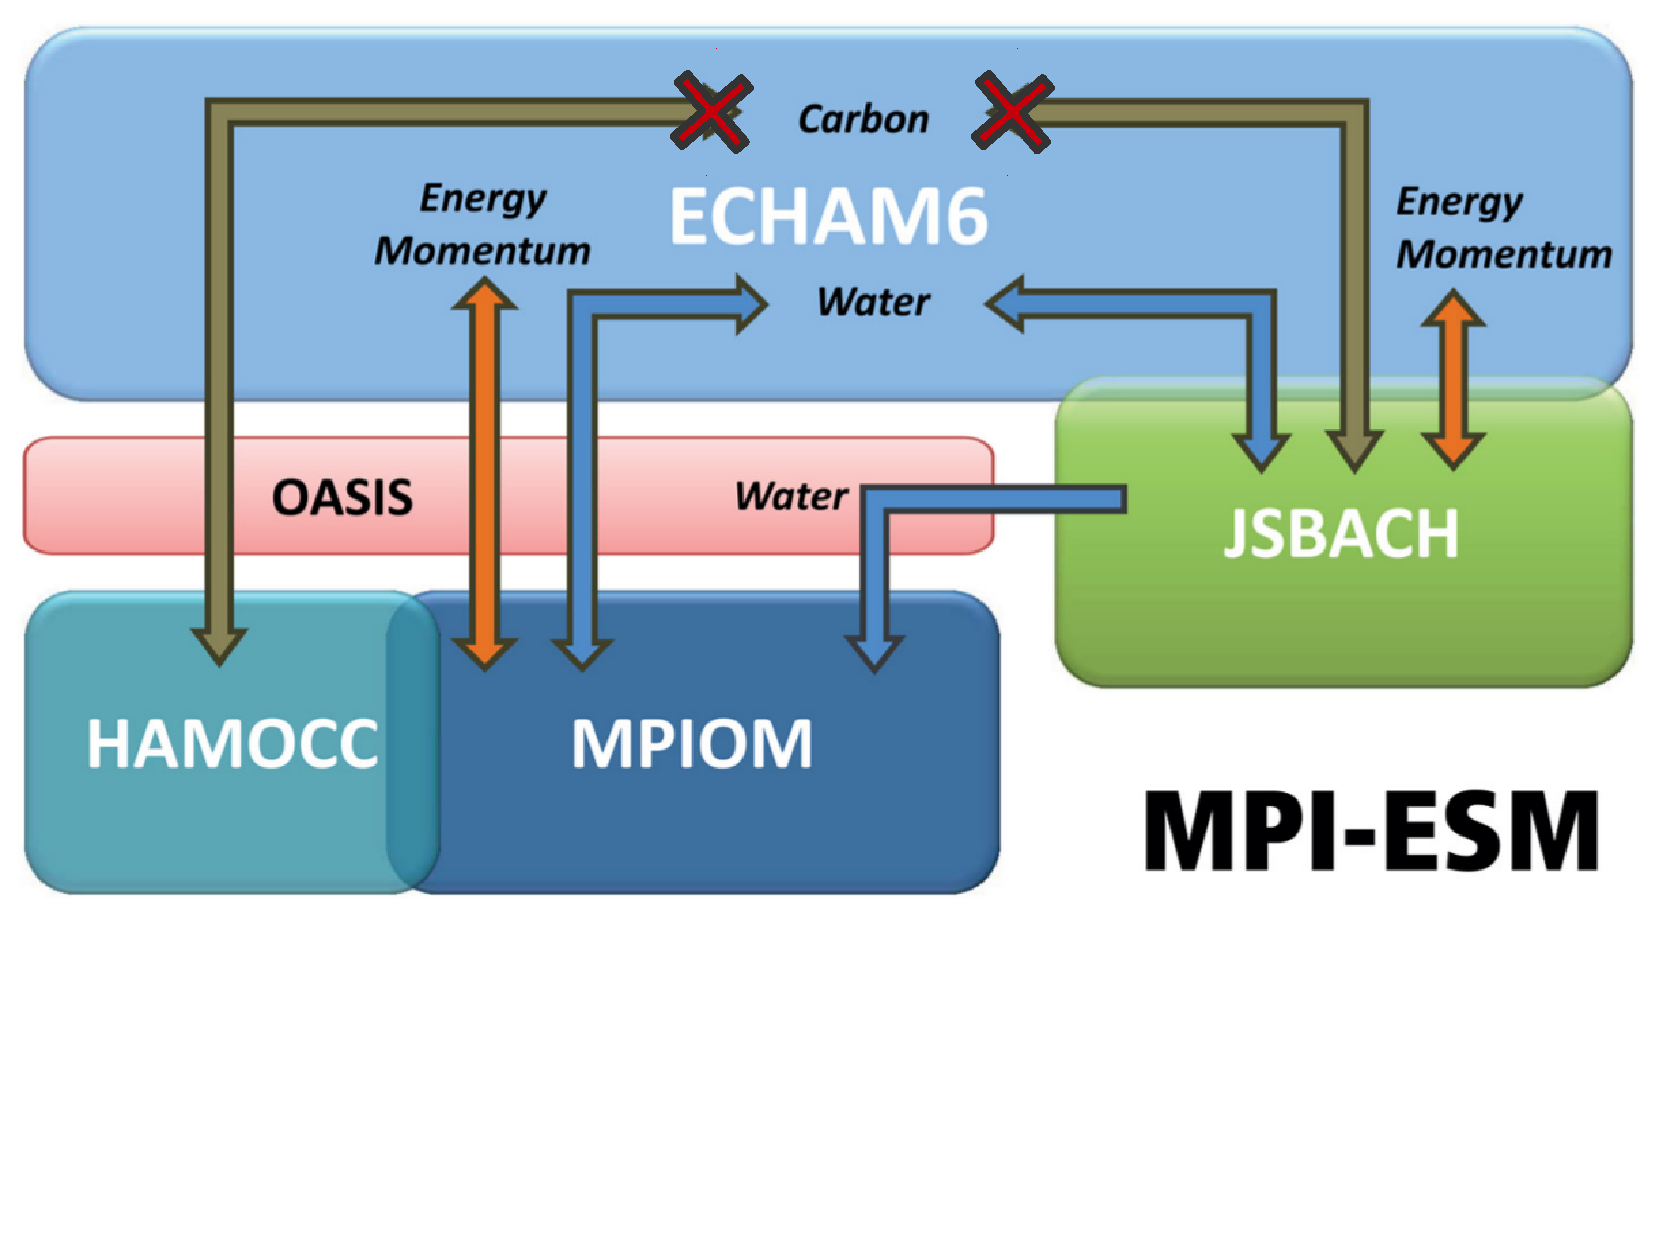
\includegraphics[scale=.28,trim=0cm 6cm 0cm 0cm,clip]{MPIESM.pdf}
		\caption{Schematic view of MPI-ESM1.1 with prescribed atmospheric pCO$_2$ \citep{Giorgetta2013}}
		\end{minipage} \hfill \pause
		\begin{minipage}{.35\textwidth}
		%\vspace{-1mm}
		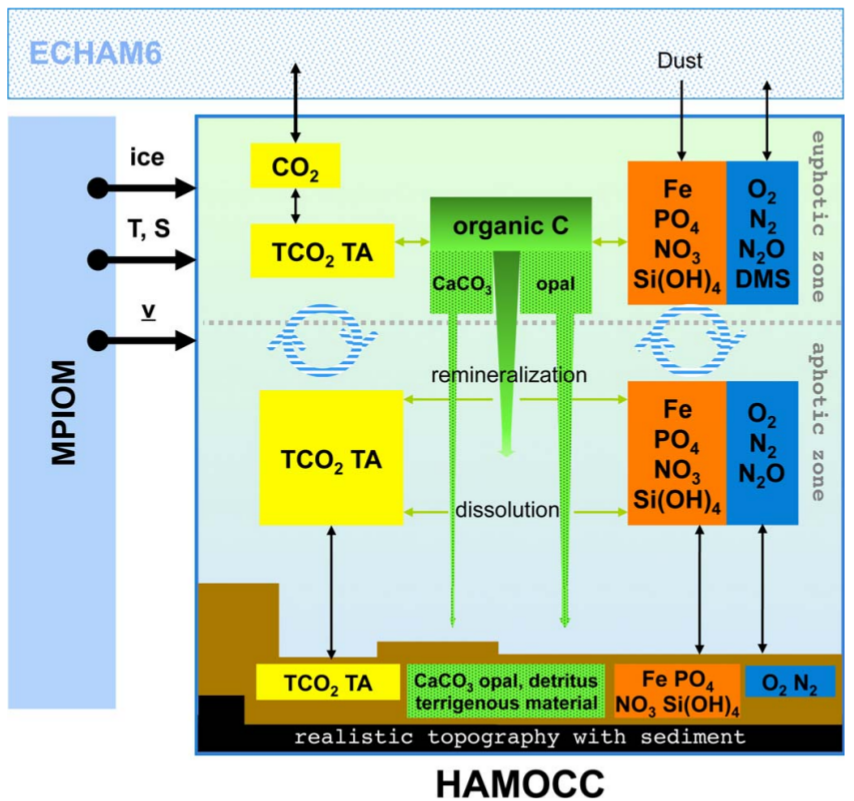
\includegraphics[scale=.2]{hamocc}	
		\vspace{-1mm}	
		\caption{Schematic view of \href{https://www.dkrz.de/about/media/galerie/Vis/esm/hamocc}{HAMOCC} \citep{Ilyina2013}}
		\end{minipage}
	\end{figure}
\end{frame}

\section{Scientific questions}
\begin{frame}{Scientific questions}
\Large
	\begin{enumerate}[<+->]
	\item How large is the modeled decadal internal variability in the Southern Ocean carbon sink?
	\item Do we find similar trends to those observed in the 1990s and 2000s in this large ensemble?
	\item Which processes drive decadal internal variability in this large ensemble?
	\end{enumerate}
\end{frame}

\begin{frame}{What is internal variability?}
\label{sec:DIV}
\vspace{-1cm}
 \begin{columns}
          \column{0.42\linewidth}
            \[ \text{signal}=\underbrace{\text{forced signal}}_{\text{ensemble mean}}+\underbrace{\text{internal variability}}_{\text{residual}}\]
			\small         
          % \[\text{CO}_2\text{flux}=k_w \cdot  \underbrace{\left( pCO_\text{2,atm} - pCO_\text{2,ocean}\right)}_{\Delta pCO_2   }\]
           \column{0.58\linewidth} 
				\begin{figure}
 					\centering
             		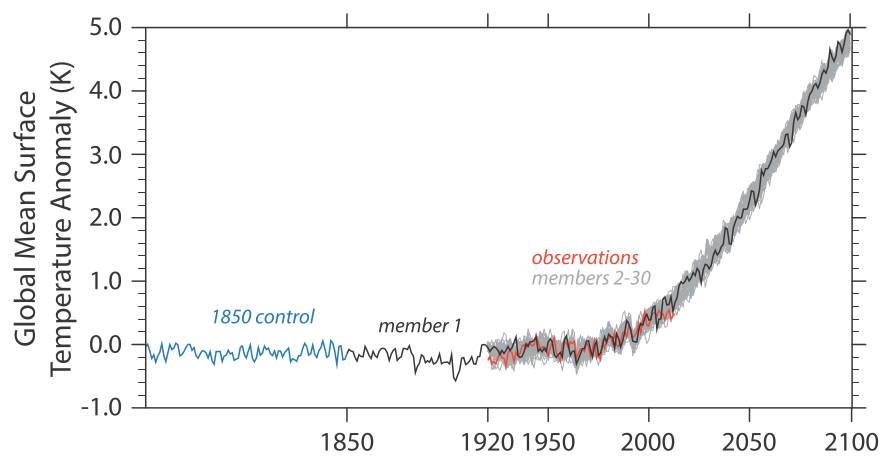
\includegraphics[scale=.32]{Kay_fig2.png}
              		\caption{Global surface temperature anomaly \citep{Kay2015}}
				\end{figure}           
         
         \end{columns} 


\pause
I define decadal internal variability $\sigma_{DIV}$ as the standard deviation of differences of the annual mean state after a decade over all $N$ ensemble members and $M$ decades.

\vspace{-2mm}
\begin{align*}
\sigma_{DIV}(X) &= \sqrt{\frac{1}{M N} \sum_{n=\text{ens}}^{N} \sum_{m=\text{yr}}^{M} \left( \chi_{m,n} -\bar{\chi}_{m,n}\right)^{2}} \hspace{12mm}
\chi_{m,n}&=X_{\text{decade}_{\text{end}},n}-X_{\text{decade}_{\text{start}},n}
\end{align*}
\end{frame}

\section{Results}
\begin{frame}{The modeled internal decadal variability $\sigma_{DIV}$ is 0.18 PgC/yr.} 
\vspace{.45cm}

\begin{figure}%[h!]
	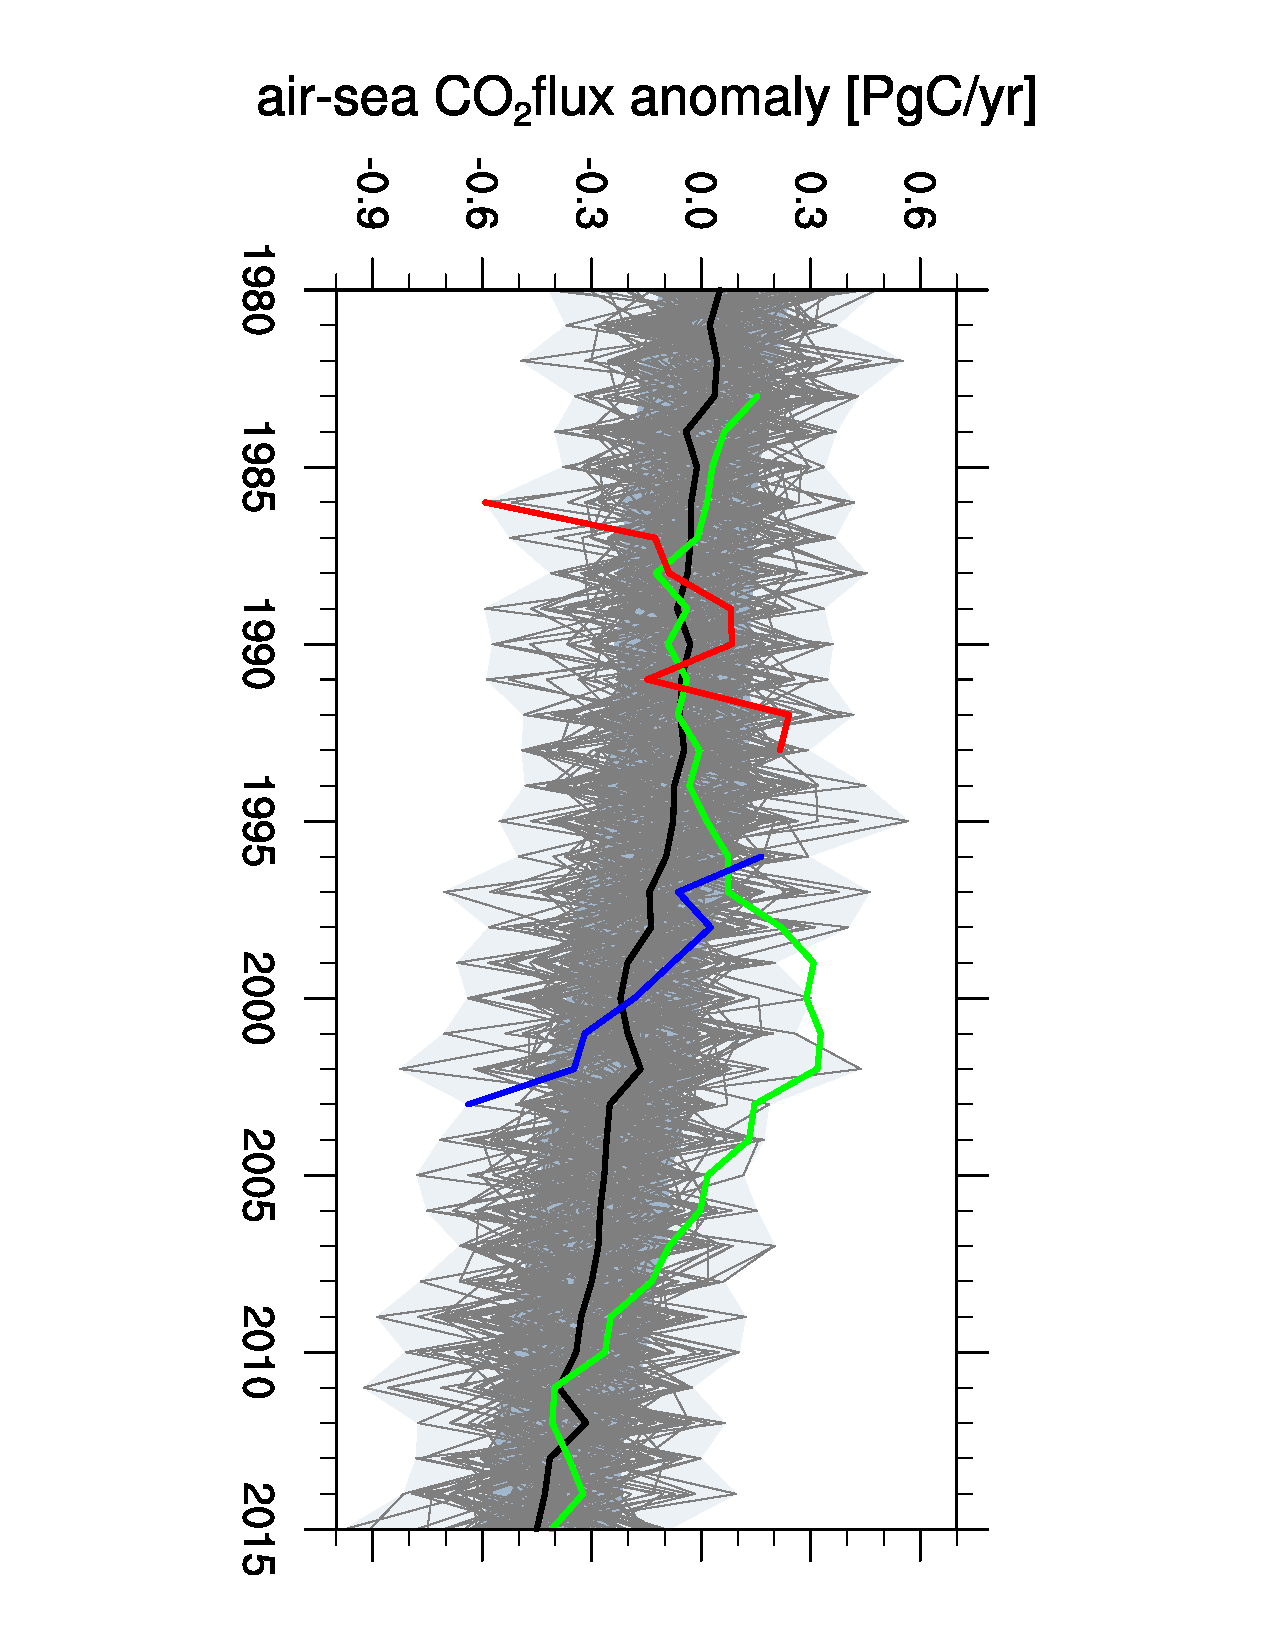
\includegraphics[scale=.4,angle=90,trim=4cm 0cm 4cm 0cm,clip]{co2flux_SO_timeseries_ymjm_35S_1980_2015_trend_8}
	\vspace{-2mm}
	\caption{Temporal evolution of the Southern Ocean air-sea CO$_2$ flux anomaly south of 35$^\circ$S. Grey lines show the 100 ensemble members, the black line the ensemble mean, the blue shading is the ensemble decadal internal variability $\sigma_{DIV}$; negative values indicate anomalous carbon uptake.}
	\label{fig:evolution_southern_ocean_carbon_sink}
\end{figure}

\end{frame}	


\begin{frame}{We find positive and negative decadal CO$_2$ flux trends similar to observations in the 1990s and 2000s.} 
\vspace{-.2cm}

\begin{figure}%[h!]
	\includegraphics[scale=.4,angle=90,page=2,trim=4cm 0cm 4cm 0cm,clip]{co2flux_SO_timeseries_ymjm_35S_1980_2015_trend_8}
	\vspace{-2mm}
	\caption{Temporal evolution of the Southern Ocean air-sea CO$_2$ flux anomaly south of 35$^\circ$S. The red line shows a positive CO$_2$ flux trend, the blue line shows a negative CO$_2$ flux trend, the green line represents the SOM-FFN observation-based estimate \citep{landschuetzer2015}.}
	\label{fig:evolution_southern_ocean_carbon_sink}
\end{figure}
\addtocounter{framenumber}{-1}
\end{frame}	



\begin{frame}{The decadal internal variability $\sigma_{DIV}$ is largest at 50-60$^\circ$S.}

\begin{figure}%[h!]
	\centering
	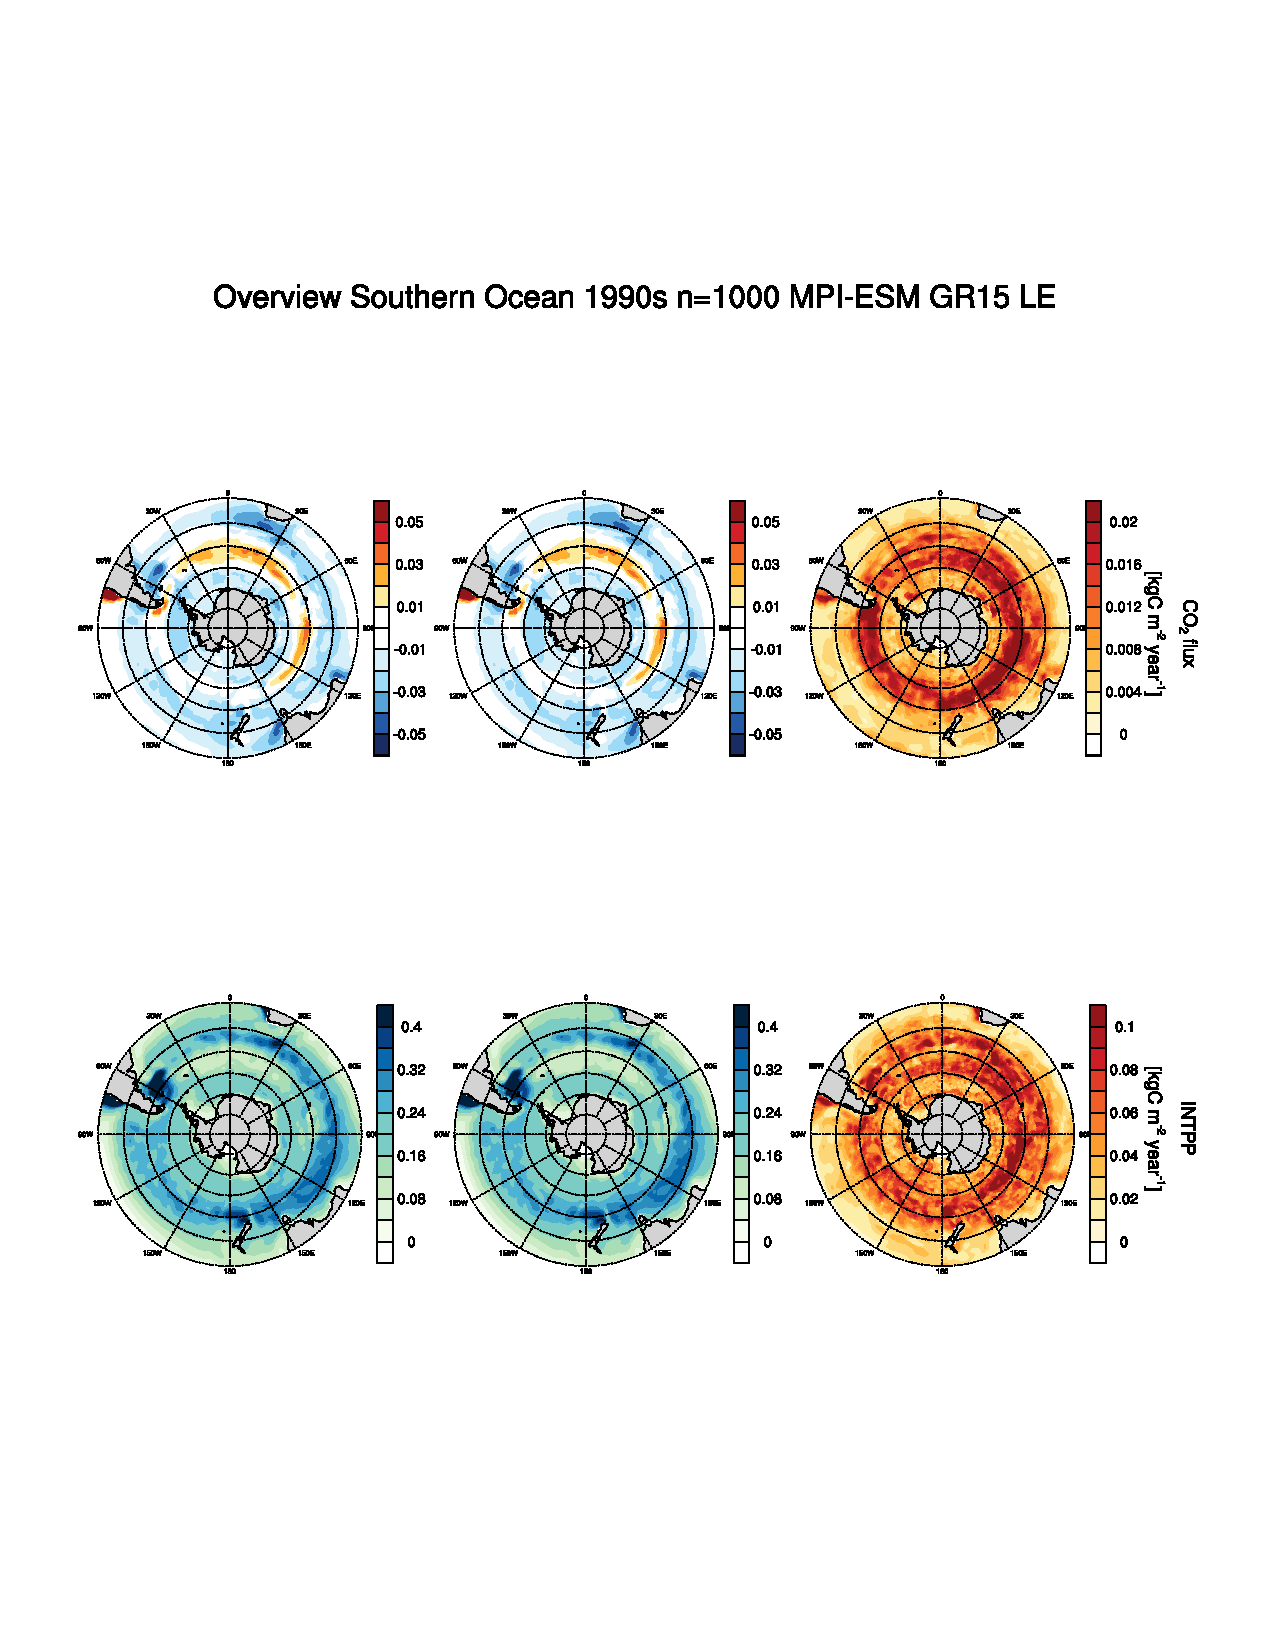
\includegraphics[scale=1.,page=1,trim=7.2cm 15cm 0cm 8cm,clip]{Overview_SO_co2flux_intpp_ens_t1990s.pdf} % co2flux
		\caption{Spatial distribution of the climatology and decadal internal variability $\sigma_{DIV}$ from 1980-2004 of the Southern Ocean air-sea CO$_2$ flux: MPI-ESM LE ensemble mean as forced signal and ensemble decadal standard deviation as decadal internal variability $\sigma_{DIV}$; negative values indicate ocean uptake.}
	\label{fig:SOCS_ensmean_ensstd}
\end{figure}

\end{frame}


\begin{frame}{We find westerly winds as the main driver of internal variability.}
\begin{figure}[h!]
\centering
%		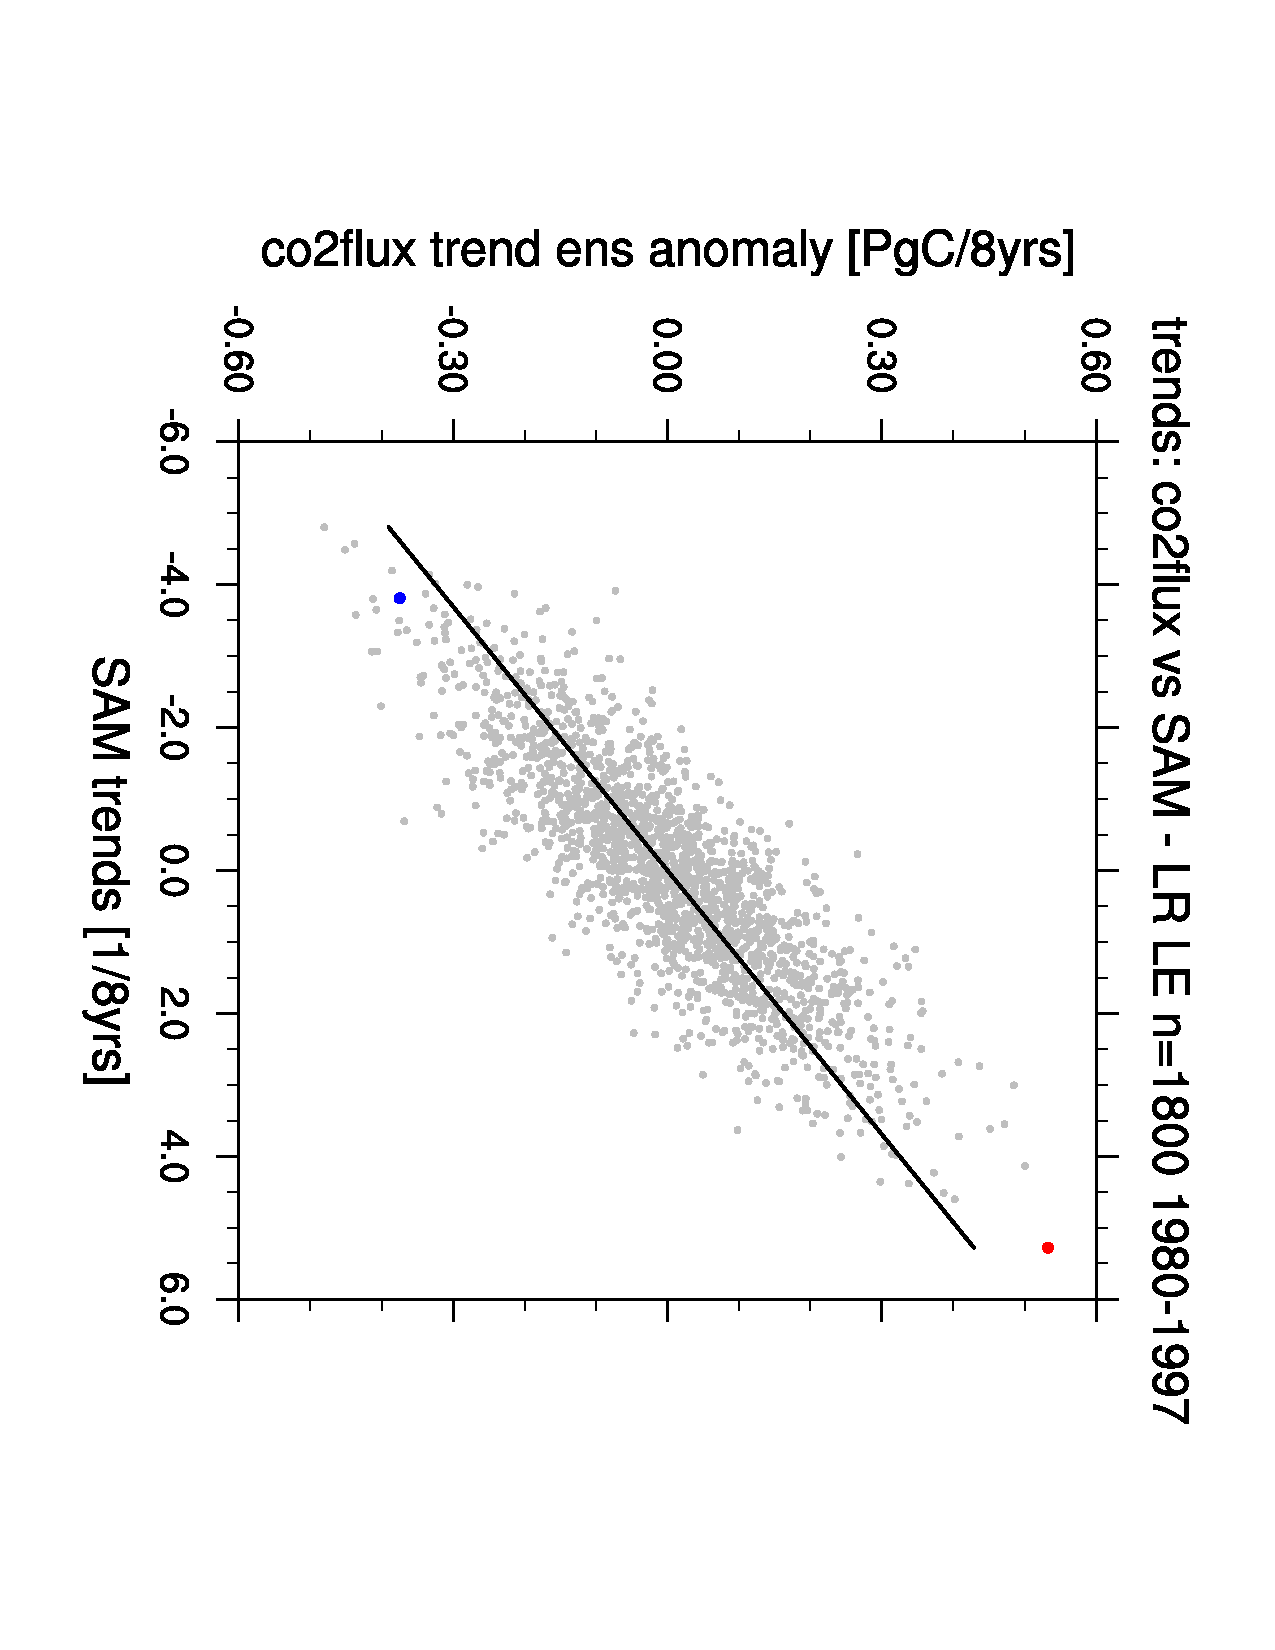
\includegraphics[scale=.5,page=1,angle=90,trim=1.3cm 2.3cm 2.3cm 3cm,clip]{Scatter_trends_bands_ensanom_co2flux_vs_SAM_n1800_1980_1997_trend8_50-59S}
		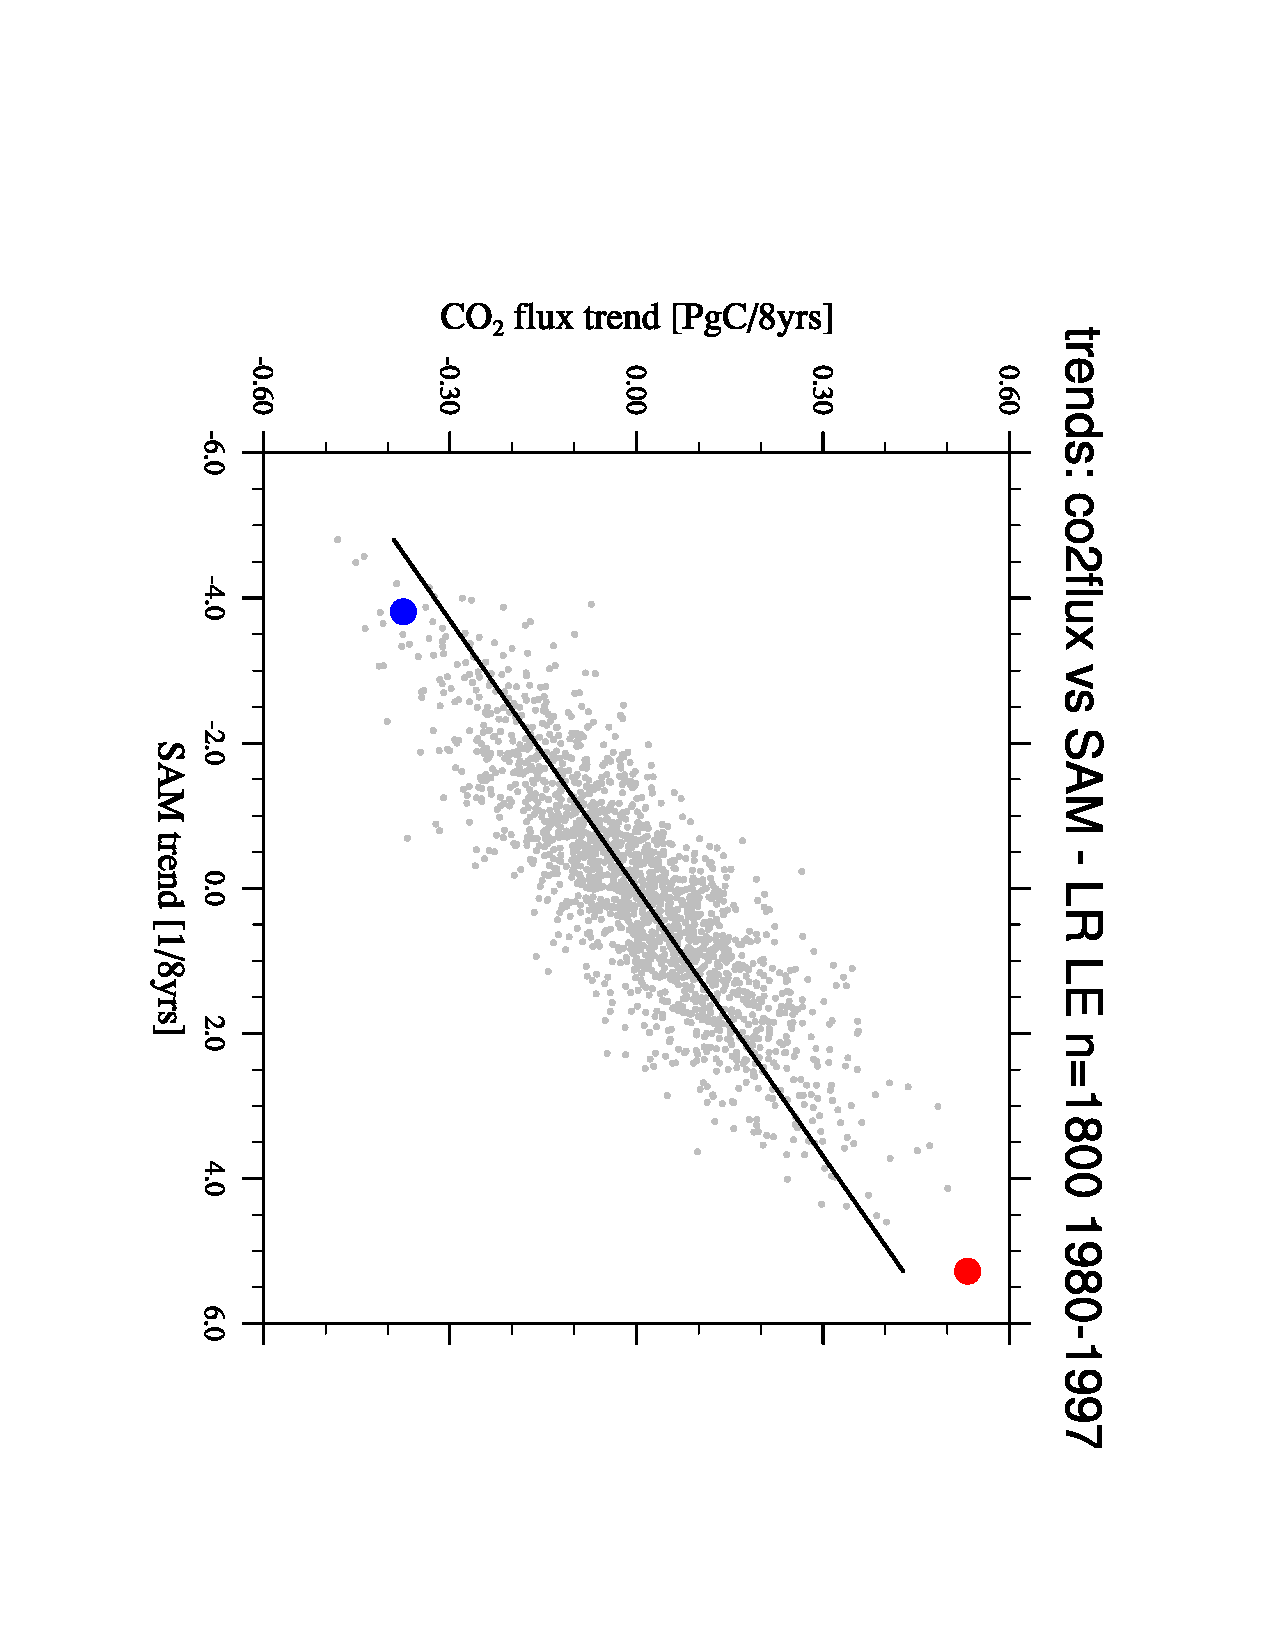
\includegraphics[scale=.34,page=1,angle=90,trim=1.3cm 2.3cm 3.8cm 3cm,clip]{EGU_new_SAM_Scatter_trends_bands_ensanom_co2flux_vs_SAM_n1800_1980_1997_trend8}
		
		%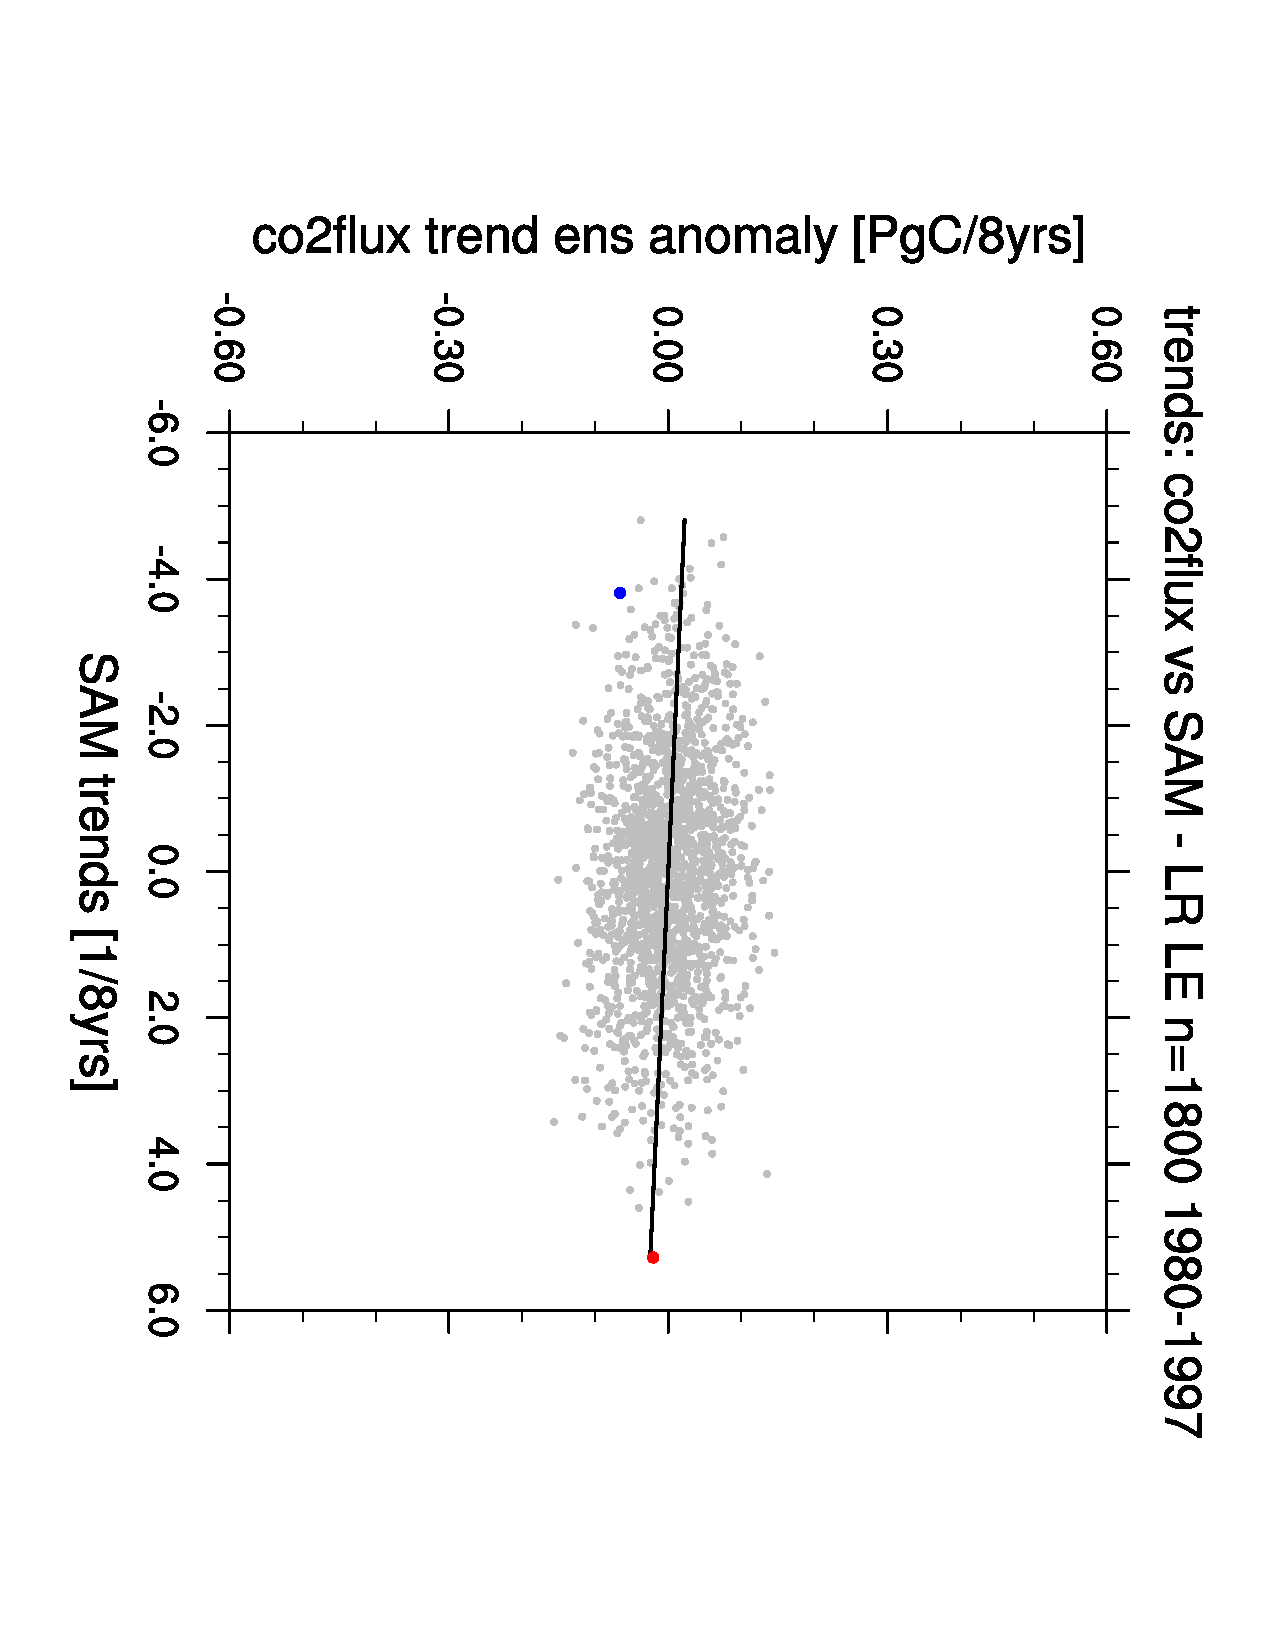
\includegraphics[scale=.38,page=1,angle=90,trim=1.3cm 2.3cm 2.3cm 3cm,clip]{Scatter_trends_bands_ensanom_co2flux_vs_SAM_n1800_1980_1997_trend8_40-49S}
		\vspace{-3mm}
		\caption{Linear trends in the Southern Annular Mode (SAM) as indicator of wind strength vs. CO$_2$ flux at 50-60$^\circ$S; each data point represents 8-year trends of a single realization normalized for the ensemble mean trend  between 1980 and 2005; the blue dot is the most negative monotonic CO$_2$ flux trend; the red dot is positive monotonic CO$_2$ flux trend.}
		\label{fig:scatter}
\end{figure}
% and analyze the response in thermal pCO$_2$ effect, biology and ocean circulation for the case of the positive CO$_2$ flux trend.
\end{frame}



\begin{frame}{Southern Ocean Review}% - Analysis of positive CO$_2$ flux trend}

\begin{figure}[h]
	\centering
	\begin{minipage}{.5\textwidth}
		\centering
			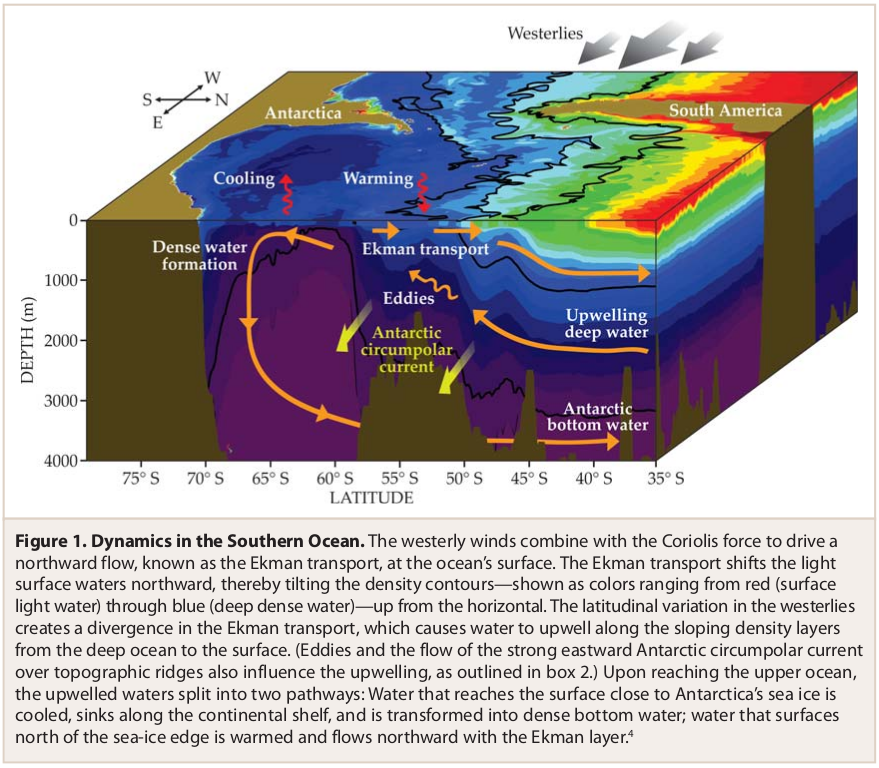
\includegraphics[scale=.35,trim=.3cm 6.8cm .5cm .5cm,clip]{Southern_Ocean_Circulation}
\vspace{-2mm}
	\caption{Dynamics of the Southern Ocean \citep{Morrison2015}}
		\label{fig:SO_review}
	\end{minipage} \hfill
	\begin{minipage}{.4\textwidth}
		%Changes in CO$_2$ flux:		
		%\begin{itemize}
		%	\item thermal
		%	\item circulation
		%	\item biology
		%\end{itemize}
		\begin{figure}[h!]
			\centering
			\includegraphics[scale=.25,trim=2cm 3.5cm 2cm 1.8cm,clip,page=14]{SO_schematics}
			\caption{Schematic illustration of the Southern Ocean under the context of increasing and southward shifted westerly winds. Red color-coding means increase, blue decrease.}
			\label{fig:schematics_neg}
		\end{figure}		
		
	\end{minipage}
\end{figure}

\end{frame}
	
%not nessessarily needed	
%\begin{frame}{Internal Variability of CO$_2$flux and primary production show similar patterns, have highest values at 45-60$^\circ$S south and appear in same locations.}  
	
%	\begin{figure}
%		\centering
%		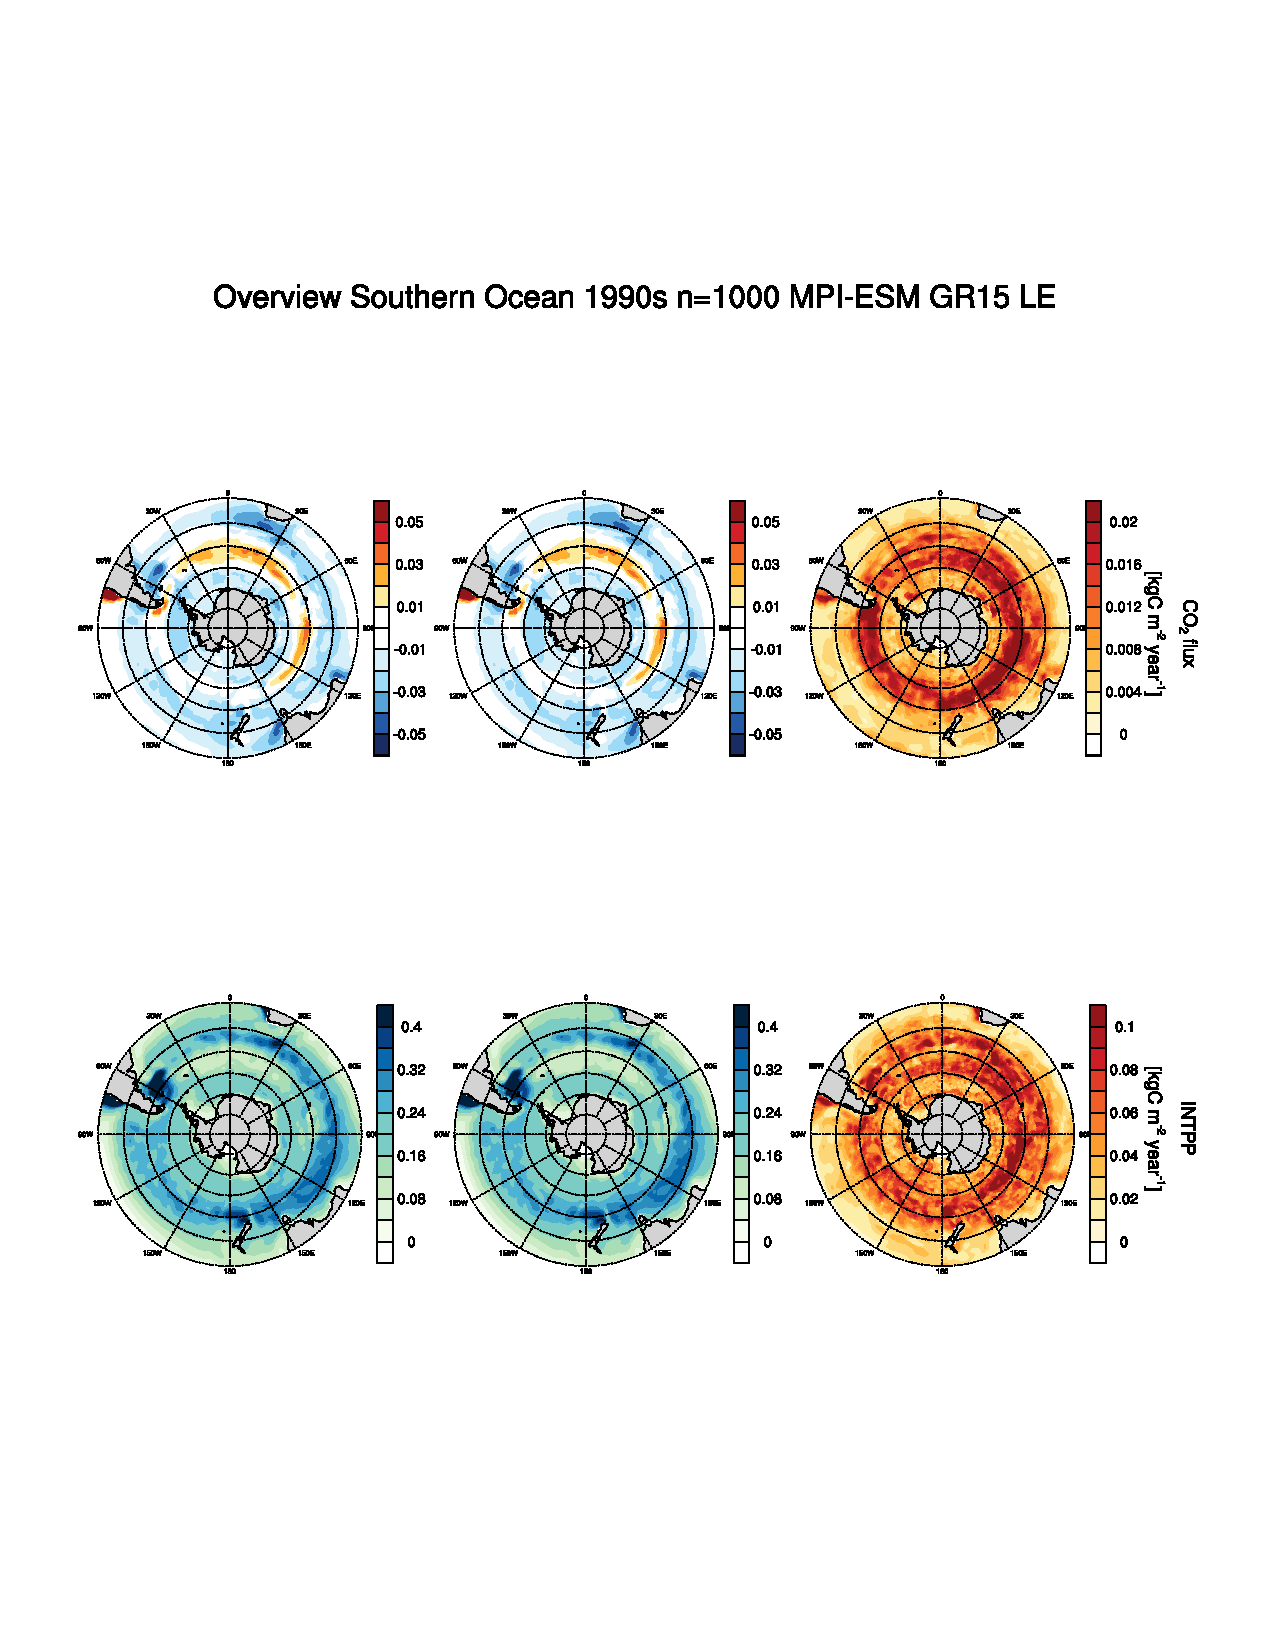
\includegraphics[scale=.45,trim=7.2cm 15cm 0cm 8cm,clip]{Overview_SO_co2flux_intpp_ens_t1990s.pdf} % from gfx folder
%		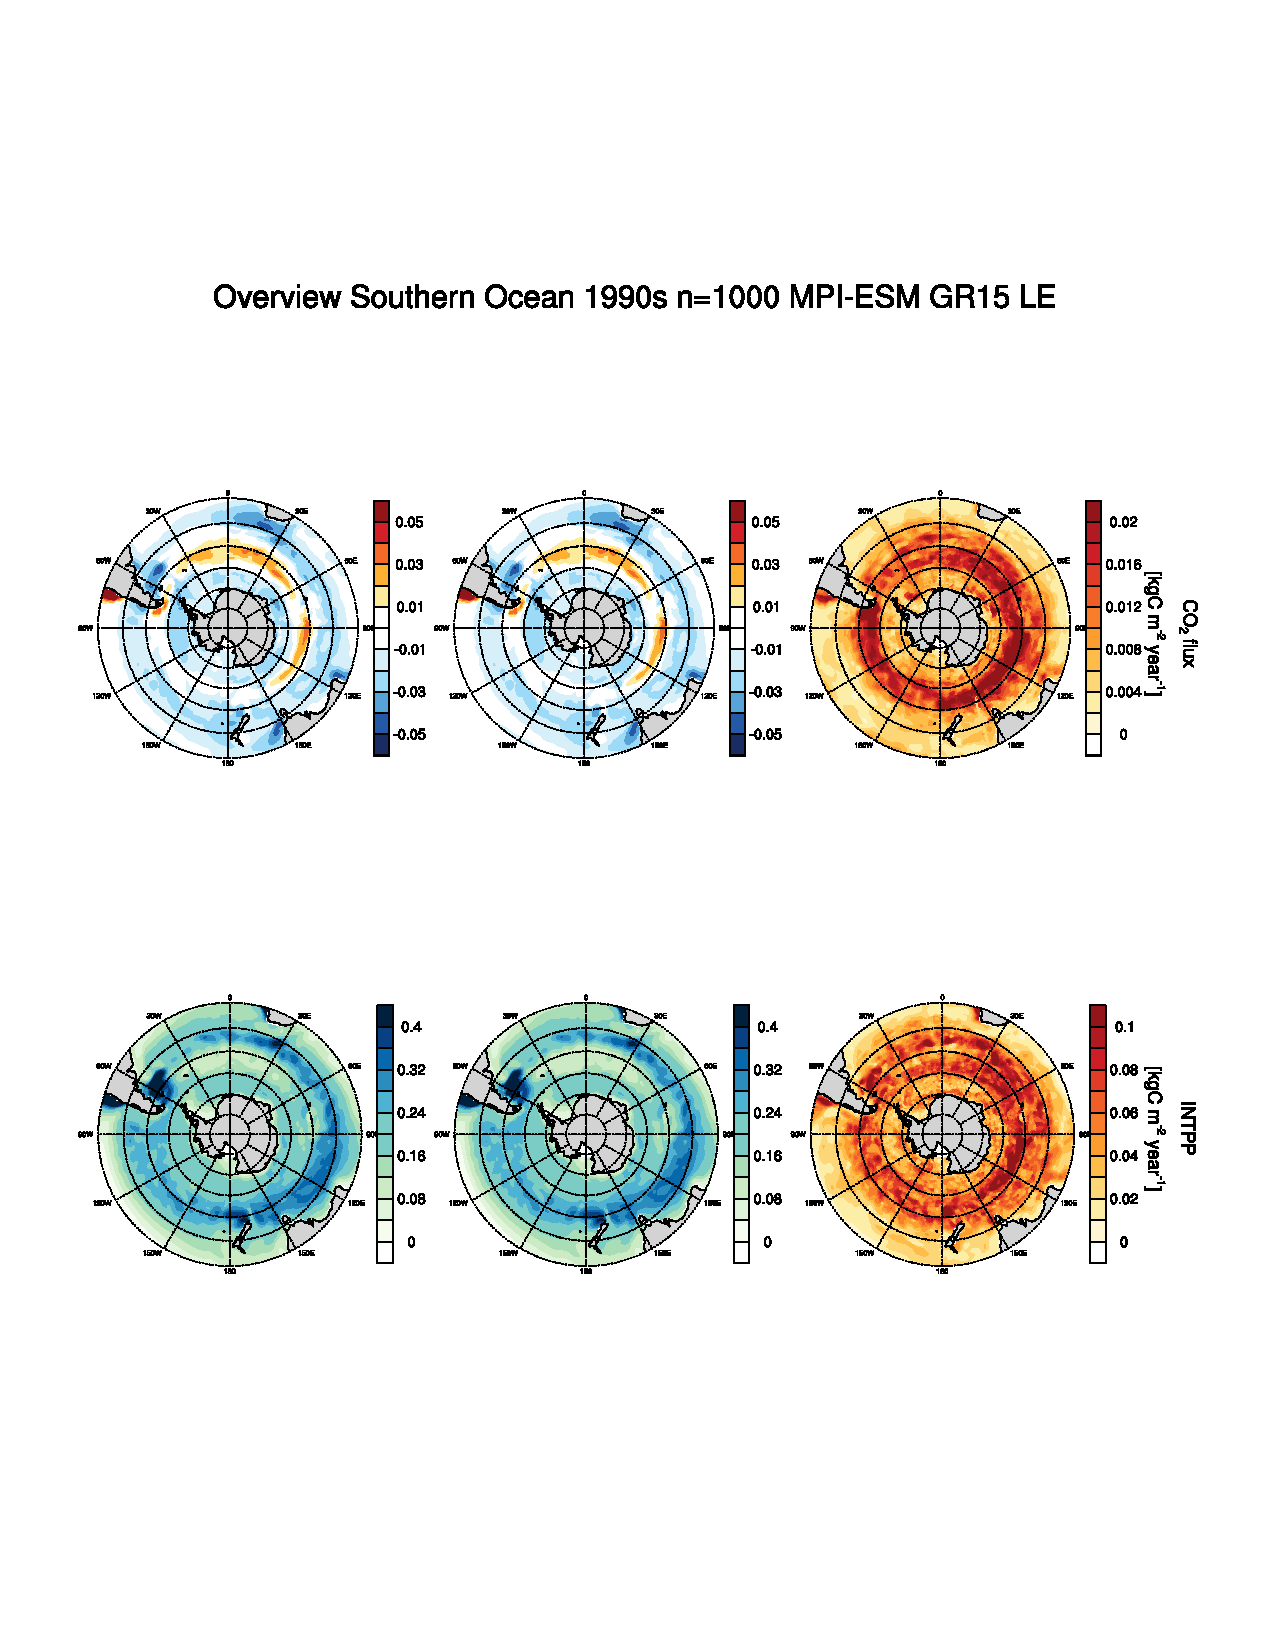
\includegraphics[scale=.45,trim=7.2cm 6.3cm 0cm 16cm,clip]{Overview_SO_co2flux_intpp_ens_t1990s.pdf} % from gfx folder
%	\caption{Southern Ocean CO$_2$flux where negative values indicate ocean uptake (1$^{st}$) and primary production (2$^{nd}$): ensemble median (left) as forced signal and ensemble standard deviation (right) as internal variability \citep{Deser2012}}
%		\label{fig:SOCS_ensmean_ensstd}
%	\end{figure}
%\end{frame}	
	
\begin{frame}{Enhanced and southward shifted westerly winds induce positive CO$_2$ flux trends. What's the response in thermal pCO$_2$, biology and ocean circulation?} %third scientific question
\vspace{-1mm}
\begin{figure}[h!]
\centering
	\includegraphics[scale=.68,trim=6.3cm 14.4cm 5.5cm 6.4cm,clip]{\memberpositive _positive_trend_8_Landschuetzer_overview.pdf}
	\includegraphics[scale=.9,trim=7.2cm 4.7cm 6.8cm 17.8cm,clip]{\memberpositive _positive_trend_8_Landschuetzer_overview.pdf}	
	\caption{Linear trends in $\Delta$pCO$_2$ (left) and sea-level pressure \& winds (right) for the case of the most positive monotonic 8-year CO$_2$ flux trend; hatched areas indicate where trends are outside the 5\% significance level}% - should I also discuss thermal and non-thermal trends in \citep{landschuetzer2015}?}
	\label{fig:pco2_pos}
\end{figure}
\note{third research question}

\end{frame}




\subsection{Thermal}
\begin{frame}{The non-thermal trend dominates over the thermal.}
%\vspace{1mm}
\begin{minipage}{.3\textwidth}
\citep{Takahashi2002}:
\end{minipage} \hfill
	\begin{minipage}{.66\textwidth}
\begin{align*}
pCO_{\text{2,thermal}}&=\overline{pCO_2} \cdot \exp \left[ 0.0423 ^{\circ}C^{-1}\left( T - \overline{T} \right) \right] \\
pCO_{\text{2,non-thermal}}&=pCO_2 \cdot \exp \left[ 0.0423 ^{\circ}C^{-1}\left( \overline{T} - T \right) \right] 
\end{align*} 
\end{minipage}
	\centering
	\begin{minipage}{.3\textwidth}
		
		\begin{figure}[h!]
			\centering
			\vspace{-1mm}
			\includegraphics[scale=.25,trim=3.5cm 3.5cm 2cm 1.95cm,clip,page=10]{SO_schematics}
			\caption{Schematic illustration of the thermal CO$_2$ flux response for increasing westerly winds}
			\label{fig:schematics_neg}
		\end{figure}		
	
		
	\end{minipage} \hfill
	\begin{minipage}{.66\textwidth}
		\begin{figure}[h!]
\centering
	\includegraphics[scale=1.0,trim=6cm 10.2cm 5.2cm 14cm,clip]{\memberpositive _positive_trend_8_Landschuetzer_overview.pdf}
	\caption{Linear trends in pCO$_{2,\text{thermal}}$ (left) and $\Delta$pCO$_{2,\text{non-thermal}}$ (right) for the case of the most positive monotonic 8-year CO$_2$ flux trend; hatched areas indicate where trends are outside the 5\% significance level}
	\label{fig:thermal_pos}
\end{figure}
	\end{minipage}
\end{frame}



\subsection{Circulation}
\begin{frame}{Upper-ocean overturning circulation is enhanced.}

	\begin{minipage}{.3\textwidth}
		
		\begin{figure}[h!]
			\centering
			\includegraphics[scale=.25,trim=3.5cm 3.5cm 7cm 1.95cm,clip,page=2]{SO_schematics}
			\caption{Schematic illustration of the circulation CO$_2$ flux response for increasing westerly winds}
			\label{fig:schematics_neg}
		\end{figure}		
	
		
	\end{minipage} \hfill
	\begin{minipage}{.66\textwidth}
		\begin{figure}[h!]
		\begin{figure}[h!]
	\centering
	\includegraphics[scale=1.,trim=13.cm 18.75cm 3cm 6cm,clip]{\memberpositive _positive_trend_8_ekman_overview.pdf}
	\includegraphics[scale=1.,trim=13.25cm 15.9cm 3cm 9.2cm,clip]{\memberpositive _positive_trend_8_ekman_overview.pdf}
	%\includegraphics[scale=0.25,page=2,trim=.3cm 1.7cm 0cm 4.6cm,clip]{UOOC}
	\caption{Linear trends in Ekman transport and Ekman pumping in the case of the most positive 8-year CO$_2$ flux trend; hatched areas indicate where trends are outside the 5\% significance level}
	\label{fig:UOOC_pos}
\end{figure}
		\end{figure}
	\end{minipage}

\end{frame}

\begin{frame}{Upper-ocean overturning circulation is enhanced and drives outgassing.}
\addtocounter{framenumber}{-1}
	\begin{minipage}{.3\textwidth}
		
		\begin{figure}[h!]
			\centering
			\vspace{-1mm}
			\includegraphics[scale=.25,trim=3.5cm 3.5cm 7cm 1.95cm,clip,page=2]{SO_schematics}
			\caption{Schematic illustration of the circulation CO$_2$ flux response for increasing westerly winds}
			\label{fig:schematics_neg}
		\end{figure}		
	
		
	\end{minipage} \hfill
	\begin{minipage}{.66\textwidth}
		\begin{figure}[h!]
		\begin{figure}[h!]
	\centering
	%\includegraphics[scale=1.,trim=13.cm 18.75cm 3cm 6cm,clip]{\memberpositive _positive_trend_8_ekman_overview.pdf}
	%\includegraphics[scale=1.,trim=13.25cm 15.9cm 3cm 9.2cm,clip]{\memberpositive _positive_trend_8_ekman_overview.pdf}
	\includegraphics[scale=0.33,page=2,trim=0cm 1.7cm 0cm 4.6cm,clip]{UOOC}
	\caption{Zonally averaged upper-ocean overturning circulation in the case of the most positive 8-year CO$_2$ flux trend; similar \citep{DeVries2017}}
	\label{fig:UOOC_pos}
\end{figure}
		\end{figure}
	\end{minipage}

\end{frame}




	
\subsection{Biology}
\begin{frame}{Primary production trends oppose CO$_2$ flux trends, but not caused by changes in nutrients.}

	\begin{minipage}{.3\textwidth}
		
		\begin{figure}[h!]
			\centering
			\includegraphics[scale=.25,trim=3.5cm 3.5cm 7cm 1.95cm,clip,page=3]{SO_schematics}
			\caption{Schematic illustration of the biological CO$_2$ flux response for increasing westerly winds}
			\label{fig:schematics_neg}
		\end{figure}		
	
		
	\end{minipage} \hfill
	\begin{minipage}{.66\textwidth}
	\begin{figure}
		\centering
		\vspace{-6mm}
		\includegraphics[scale=.88,trim=13.25cm 18.7cm 2.5cm 6.4cm,clip]{\memberpositive _positive_trend_8_obgc_overview_summer.pdf} %co2flux
\includegraphics[scale=.88,trim=13.25cm 15.9cm 2.5cm 9.2cm,clip]{\memberpositive _positive_trend_8_obgc_overview_summer.pdf} %intpp

\includegraphics[scale=.88,trim=13.25cm 13.1cm 2.5cm 12.1cm,clip]{\memberpositive _positive_trend_8_obgc_overview_summer.pdf} %nutlimf
\includegraphics[scale=.88,trim=13.25cm 7.3cm 2.5cm 17.8cm,clip]{\memberpositive _positive_trend_8_obgc_overview_summer.pdf} %zmld
\caption{Southern Ocean austral summer trends over 8 years: CO$_2$flux (top left), vertically integrated primary production (top right), surface nutrient limitation (bottom left) and mixed layer depth (bottom right); hatched areas indicate where trends are outside the 5\% significance level}
\label{fig:co2flux_intpp}
	\end{figure}
		\end{minipage}
\end{frame}	

\begin{frame}{Light \& temperature limitation causes the decline in primary production at 50-60$^\circ$S. Phytoplankton gets mixed deeper into the ocean.} %\citep{Sverdrup1953}.}
%\hspace{-3mm}
	\begin{figure}
		\centering
		\includegraphics[scale=1.,trim=13.2cm 15.9cm 3.4cm 9.2cm,clip]{\memberpositive _positive_trend_8_schwerpunkt_mixing_overview.pdf} % wind penetration depth	
	\includegraphics[scale=1.,trim=13.2cm 18.7cm 3.4cm 6.4cm,clip]{\memberpositive _positive_trend_8_schwerpunkt_mixing_overview.pdf} % phy depth	
		\includegraphics[scale=1.,trim=13.2cm 4.5cm 3.4cm 20.65cm,clip]{\memberpositive _positive_trend_8_obgc_overview_summer.pdf} %light_temp	

\caption{Trends in of average depth of vertical diffusivity due to wind (left), phytoplankton average depth (middle) and surface light \& temperature limitation factor; hatched areas indicate where trends are outside the 5\% significance level}
\label{fig:wind_mixing}
	\end{figure}
	
\end{frame}



\begin{frame}{Previous studies show increasing primary production for increasing winds. Increased upwelling brings more nutrients, but this has no effect on biology in HAMOCC. However, biology signal much smaller than circulation.}
\begin{figure}
\centering
\vspace{-.5cm}
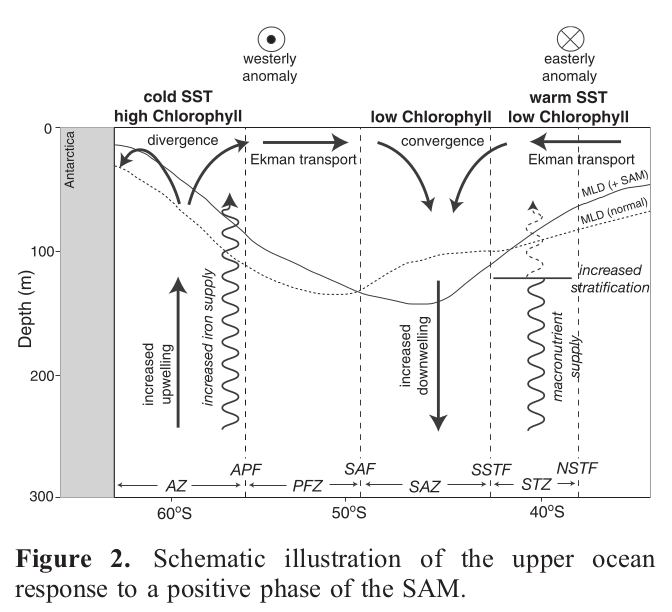
\includegraphics[scale=.3,trim=0cm 2.3cm 0cm .7cm,clip]{Southern_Ocean_SAM_zmld_response_Lovenduski2005}
\includegraphics[scale=1.1,trim=5.8cm 13.1cm 12cm 12.1cm,clip]{\memberpositive _positive_trend_8_obgc_overview_summer.pdf} %nutlimf
\includegraphics[scale=1.1,trim=13.25cm 13.1cm 3.3cm 12.1cm,clip]{\memberpositive _positive_trend_8_obgc_overview_summer.pdf} %nutlimf
\caption{(left) Schematic view of the upper ocean
response to a positive SAM phase \citep{Lovenduski2005}; (right) surface nutrient limitation function summer mean and trend} 
\end{figure}
\vspace{-3mm}
related papers: \citep{Lovenduski2008} \citep{wang2012} \citep{Hauck2013} 
\end{frame}

\begin{frame}{Intensified winds reduce the overall Southern Ocean carbon sink.}
	\begin{minipage}{.32\textwidth}		
		
		\begin{table}
		\begin{tabular}{l l}
		thermal & - \\
		circulation & + \\
		biology & + \\ \hline
		total & +
		\end{tabular}		
		\end{table}
			\end{minipage} \hfill
	\begin{minipage}{.65\textwidth}	
	
	\begin{figure}[h!]
			\centering
			
			\includegraphics[scale=.45,trim=3.5cm 3.5cm 7cm 1.95cm,clip,page=12]{SO_schematics}		
			\label{fig:schematics_neg_all}
		\end{figure}	
		\end{minipage}

\end{frame}


\section{Summary}
\begin{frame}{Summary}
	\begin{minipage}{.23\textwidth}
		
		\begin{figure}[h!]
			\centering
			
			\includegraphics[scale=.15,trim=3.5cm 3.5cm 7cm 1.95cm,clip,page=12]{SO_schematics}
			
			\includegraphics[scale=.15,trim=3.5cm 3.5cm 7cm 1.95cm,clip,page=13]{SO_schematics}
			
			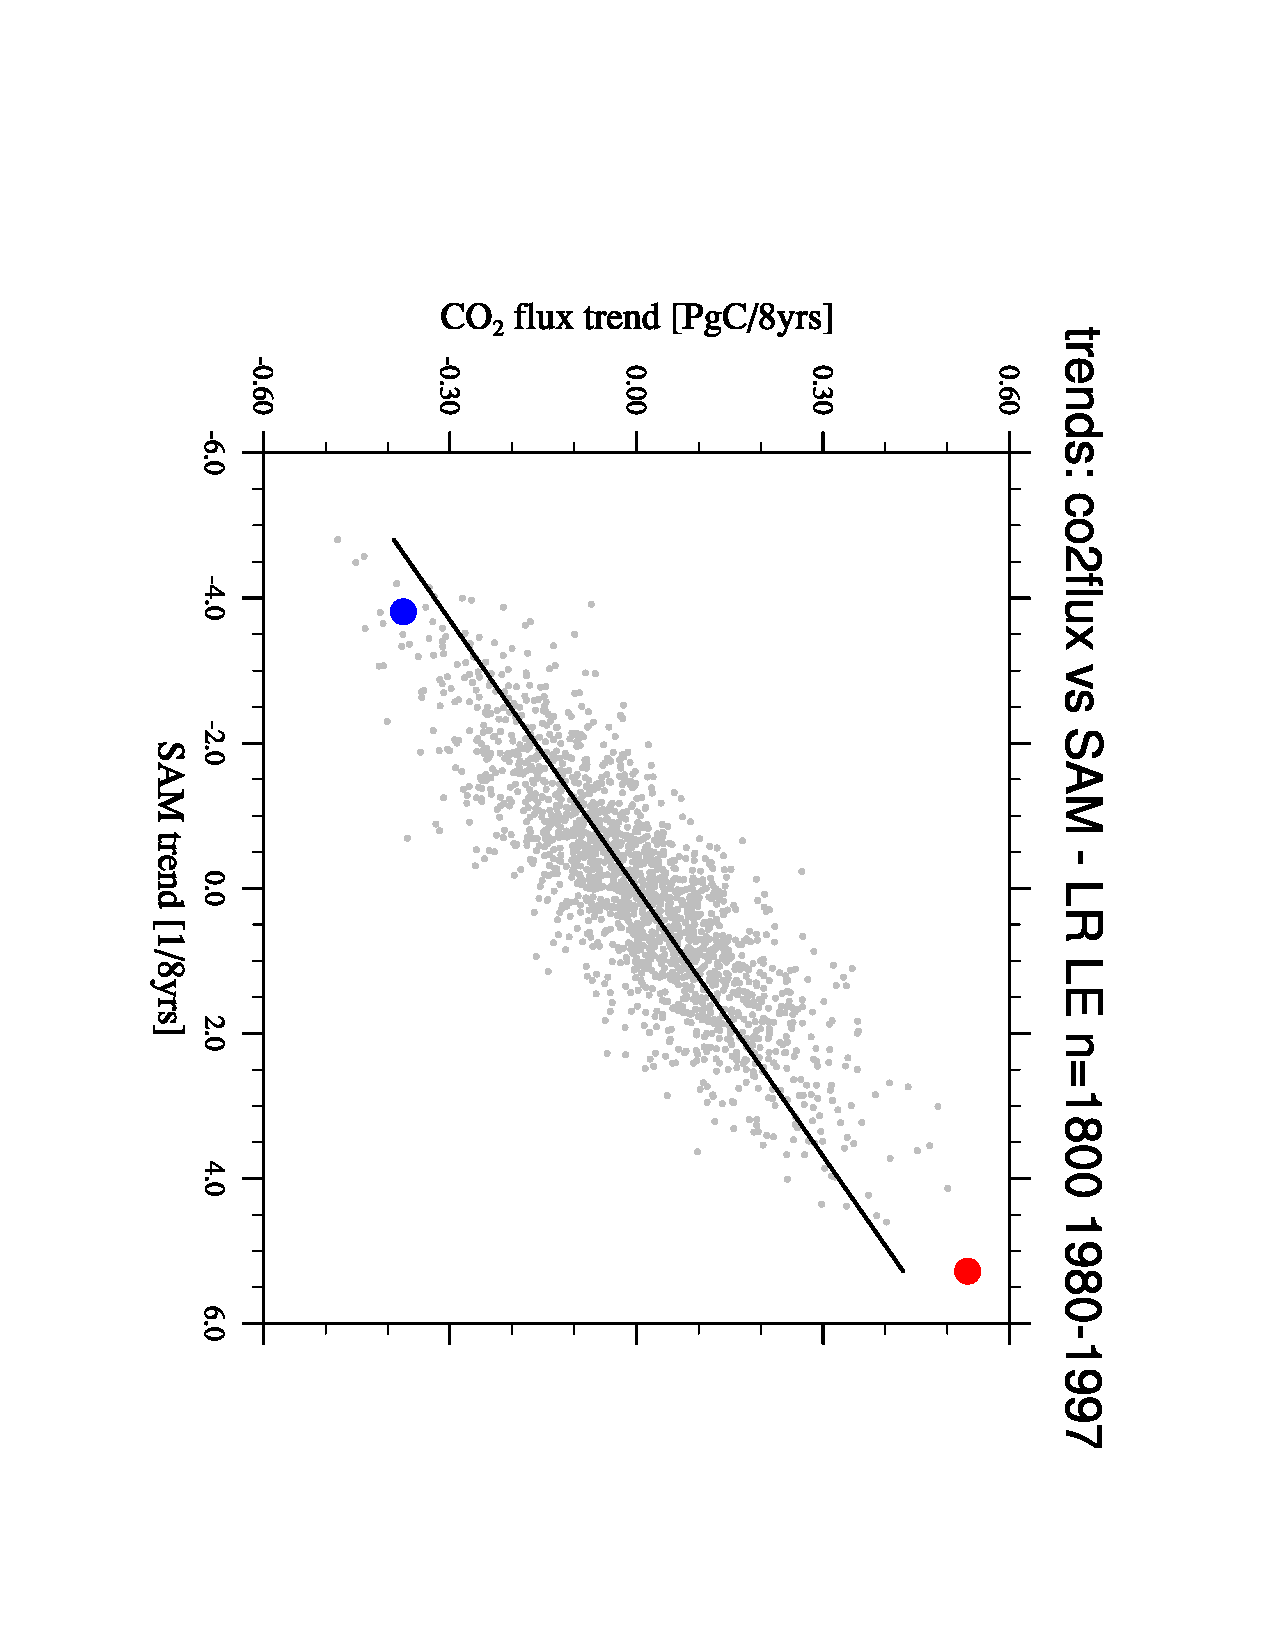
\includegraphics[scale=.15,page=1,angle=90,trim=1.3cm 2.3cm 3.8cm 3cm,clip]{EGU_new_SAM_Scatter_trends_bands_ensanom_co2flux_vs_SAM_n1800_1980_1997_trend8}
			
			\caption{Schematic illustration of the Southern Ocean for the CO$_2$ flux response for increasing westerly winds}
			\label{fig:schematics_neg}
		\end{figure}		
	
		
	\end{minipage} \hfill
	\begin{minipage}{.75\textwidth}
	\vspace{-30mm}
\begin{itemize}[<+->]
\item Modeled decadal internal variability $\sigma_{DIV}\approx 0.18$ PgC/yr and is largest at 50-60$^\circ$S
\item MPI-ESM Large Ensemble captures multi-year positive and negative trends as suggested by observations
\item Trends reverse for decreasing winds
\item We find two wind-driven regimes of the Southern Ocean carbon sink: Enhanced winds... 
\begin{itemize}
\item increase thermal CO$_2$ uptake
\item increase upwelling
\item decrease primary production
\end{itemize}

Overall, this weakens the carbon sink and vice versa strengthens for weaker winds.

\end{itemize}
\end{minipage}

\end{frame}



\begin{frame}{Appendix}
%\appendix
\addtocounter{framenumber}{-1}
\end{frame}

\appendix

\begin{frame}{Earth-system-modeling}

\begin{figure}[h]
	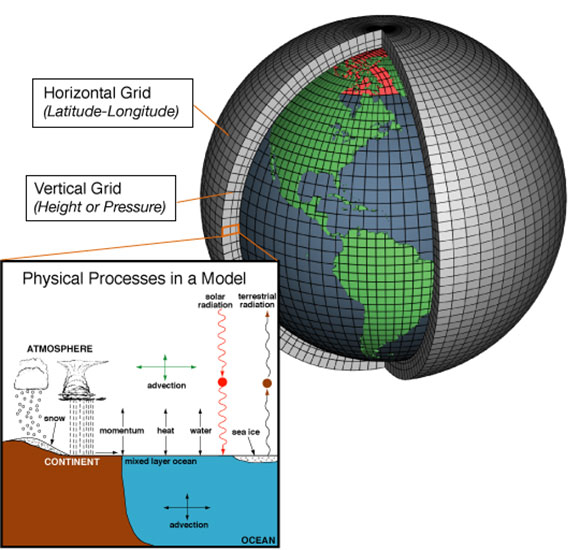
\includegraphics[scale=.3,angle=0]{AtmosphericModelSchematic.jpg} % from gfx folder
	%\includegraphics[scale=.64,angle=90,trim=1.3cm 1.3cm 5cm 1cm,clip]{heatmap_de-ens-trended.pdf} % from gfx folder
%\caption{Southern Ocean carbon sink trends per trendlength}
	\label{fig:heatmap}
\end{figure}

HAMOCC Visualisation: \url{https://www.dkrz.de/about/media/galerie/Vis/esm/hamocc}

\end{frame}



\begin{frame}{Earth-system-model scales}

\begin{figure}[h]
	\includegraphics[scale=.34,angle=0]{ESM_scales} % from gfx folder
	%\includegraphics[scale=.64,angle=90,trim=1.3cm 1.3cm 5cm 1cm,clip]{heatmap_de-ens-trended.pdf} % from gfx folder
%\caption{Southern Ocean carbon sink trends per trendlength}
	\label{fig:heatmap}
\end{figure}

\end{frame}

\begin{frame}{Earth-system-model processes}

\begin{figure}[h]
	\includegraphics[scale=.4,angle=0]{climate_models_processes.png} % from gfx folder
	%\includegraphics[scale=.64,angle=90,trim=1.3cm 1.3cm 5cm 1cm,clip]{heatmap_de-ens-trended.pdf} % from gfx folder
%\caption{Southern Ocean carbon sink trends per trendlength}
	\label{fig:heatmap}
\end{figure}

\end{frame}

		

\begin{frame}{CO$_2$ flux Southern Ocean Trendmap}
\begin{figure}[h]
	\includegraphics[scale=.38,angle=90,trim=1.4cm 1.3cm 3.5cm 1cm,clip]{heatmap_not_de-ens-trended.pdf} % from gfx folder
	%\includegraphics[scale=.64,angle=90,trim=1.3cm 1.3cm 5cm 1cm,clip]{heatmap_de-ens-trended.pdf} % from gfx folder
\caption{Southern Ocean carbon sink trends per trendlength}
	\label{fig:heatmap}
\end{figure}
\end{frame}

\begin{frame}{Model Evaluation - CO$_2$ flux}
	\begin{figure}%[h!]
	\centering
%	\llap{ \parbox[b]{0cm}{\textbf{a}\\\rule{0ex}{0cm}}}
%	\hspace{3cm} \llap{ \parbox[b]{2cm}{\textbf{b}\\\rule{0ex}{0cm}}}
	\includegraphics[scale=.52,page=1,trim=7.2cm 15cm 0cm 8cm,clip]{Overview_SO_co2flux_intpp_ens_t1990s.pdf} % co2flux
	\includegraphics[scale=.52,page=2,trim=7.2cm 15cm 0cm 8cm,clip]{Overview_SO_co2flux_intpp_ens_t1990s.pdf} % co2flux Landschuetzer
	\caption{Spatial distribution of the climatology (a,c) and decadal internal variability $\sigma_{DIV}$ (b,d) from 1980-2004 of the Southern Ocean air-sea CO$_2$ flux: MPI-ESM LE ensemble mean as forced signal (a), ensemble decadal standard deviation as decadal internal variability $\sigma_{DIV}$ (b), SOM-FFN climatology 1982-2004 (c), SOM-FFN decadal variability $\sigma_{DIV}$ (d); negative values indicate ocean uptake.}
	\label{fig:SOCS_ensmean_ensstd}
\end{figure}

\end{frame}


\begin{frame}{Model Evaluation - Winds}
\begin{figure}[h!]
	\centering
%	\llap{ \parbox[b]{0cm}{\textbf{a}\\\rule{0ex}{0cm}}}
%	\hspace{3cm} \llap{ \parbox[b]{2cm}{\textbf{b}\\\rule{0ex}{0cm}}}
	\includegraphics[scale=.52,trim=7.3cm 16.2cm 0cm 6.9cm,clip]{Overview_SO_slp_ens_t1990s.pdf} % echam
	\includegraphics[scale=.52,trim=7.3cm 10.6cm 0cm 12.5cm,clip]{Overview_SO_slp_ens_t1990s.pdf} % ncep
	\caption{Spatial distribution of the Southern Ocean sea-level pressure and winds: ensemble mean climatology from 1980 to 2004 (a) as forced signal and ensemble decadal standard deviation (b) as decadal internal variability $\sigma_{DIV}$; and the difference between MPI-ESM and reanalysis data from NCEP climatology (c), and decadal internal variability $\sigma_{DIV}$ from NCEP climatology (d).}
	\label{fig:SO_winds_ensmean_ensstd}
\end{figure}
\end{frame}

\begin{frame}{Model Evaluation - Nutrients}
\begin{figure}[h!]
	\centering
	\includegraphics[scale=.7,page=3,trim=1.8cm 13.3cm .8cm 6.5cm,clip]{Overview_SO_nutrient_comparison.pdf} % nitrate
	\caption{Spatial distribution of the climatology of surface nitrate (left) compared with WOA data \citep{WOA2013} (right)}
	\label{fig:SO_comp_nitrate}
\end{figure}
\end{frame}

\begin{frame}{Model Evaluation - SST}
\begin{figure}[h!]
	\centering
	\includegraphics[scale=.7,page=2,trim=1.8cm 13.3cm .8cm 6.5cm,clip]{Overview_SO_MPIOM_comparison.pdf} % zmld
	\caption{Spatial distribution of the ensemble mean climatology (1980-2004) of the sea-surface temperature (SST) (left) compared with xyz}
	\label{fig:SO_comp_sst}
\end{figure}
\end{frame}

\begin{frame}[allowframebreaks]{References}
\baselineskip12pt
\bibliography{../Paper/SouthernOceanCarbonSink_new}

\bibliographystyle{abbrvnat}%unsrtnat}%abbrvnat}%plainnat}

\end{frame}	
	
	
	
\end{document}